\documentclass[lang=cn,a4paper,newtx,bibend=bibtex]{elegantpaper}
\usepackage{env}
\addbibresource[location=local]{reference.bib}

\title{\emph{《有限差分法求解二维 Poisson 方程》}项目文档}
\author{张志心~~3210106357~~计科2106}
\date{Mar. 12. 2024}

\begin{document}
\maketitle

\tableofcontents
\newpage

\begin{abstract}

  该程序包为二维正方形区域 Poisson 方程的求解器,
  采用有限差分法,支持 Dirichlet,Neumann,以及混合
  边值条件问题。
  在此基础上,以从正方形区域中去掉一个圆形为例,
  该程序包实现了一种支持不规则边界的有限差分求解方法。

  该程序包中方程组的求解的部分采用了对于稀疏矩阵
  特殊优化后的LU分解法(高斯消元),
  时间复杂度仅为 $O(n^2)$,其中 $n$ 为网格的格点数。
  
  该程序包进行了充分的测试,对于二维 Poisson 方程形式的边值
  问题,达到了二阶的收敛阶。
  
  
\end{abstract}

\section{用户文档}

该部分介绍用户使用此程序包求解二维 Poisson 方程的方法。

\subsection{问题输入格式与规约}
用户需使用 \href{https://www.json.org/json-en.html}{JSON} 格式描述待求解问题(二维 Poisson 方程),
问题的数学形式为:
\[
    - \Delta u = f, \text{in~~} (\Omega \fxg D)^{\circ}
\]
其中 $\Omega = [x_l, x_r] \times [y_l, y_r] (x_r - x_l = y_r - y_l)$;
$D$ 要么为 $\emptyset$,要么为 $\{(x, y) : (x - x_c)^2 + (y-y_c)^2 \le R^2\}$。

对于边值条件,有如下几种类型:
\begin{enumerate}
  \item Dirichlet 边值条件:$u = g, \text{on~~} \partial  (\Omega \fxg D)$;
  \item Nuemann 边值条件:$\bm{n} \cdot \nabla u = g, \text{on~~} \partial  (\Omega \fxg D)$;
  \item mixed 边值条件:$\begin{cases} u = g_1 & \text{on~~} X_1 \\ \bm{n} \cdot \nabla u = g_2 & \text{on~~} X_2\end{cases}, \bigg(X_1 \cap X_2 = \emptyset, X_1 \cup X_2 = \partial (\Omega \fxg D)\bigg)$。
\end{enumerate}

\subsubsection{手动构造输入数据}

JSON 具体格式如下:
\begin{itemize}
  \item \lstinline{Domain_Border}:问题定义域外边界,格式为 $[x_l, x_r, y_l, y_r]$,
  表示 $[x_l, x_r] \times [y_l, y_r]$,若用户未定义,则默认为 $[0, 1]^2$。
  程序会检查输入外边界是否是一个合法的正方形。
  \item \lstinline{Domain_Type}:问题定义域的类型,包括 \lstinline{Regular}, \lstinline{Irregular}。
  \item \lstinline{Center}:若问题定义域是非规则类型,则需要提供内部挖去圆形的信息,圆心坐标格式为 $[x_c, y_c]$。
  \item \lstinline{R}:同上,圆形的半径为 $R$,程序会检查圆形是否位于外边界正方形的\textbf{内部}。
  \item \lstinline{Grid_n}:用户自定义网格的大小,程序会检查 $2 \le Grid\_n \le 248$,程序离散化的格点为 $(x_i, y_j) = (x_l + ih, y_l + jh), h = \frac1{Grid\_n}, i, j = 0, 1, \dots, Grid\_n$。
  \item \lstinline{BC_Type}:Poisson 方程的边值条件的类型,包括 \lstinline{Dirichlet}, \lstinline{Neumann},\lstinline{mixed}。
  \item \lstinline{f}:描述 $- \Delta u = f, \text{in~~} (\Omega \fxg D)^{\circ}$,
                       用 C++ 数学表达式的格式给出,表达式解析的具体方法见 \\
                       \texttt{/include/function\_generator/ExecCode2.hpp}。
  \item \lstinline{g}:描述 Dirichlet 边值条件($u = g, \text{on~~} \partial  (\Omega \fxg D)$)
                       或 Neumann 边值条件($\bm{n} \cdot \nabla u = g, \text{on~~} \partial  (\Omega \fxg D)$),
                       注意混合边值条件不使用该项来描述,
                       输入为一个 \texttt{JSON class},包含:
                       \begin{itemize}[$\circ$]
                        \item down : $y = y_l$ 上边值条件表达式;
                        \item left : $x = x_l$ 上边值条件表达式;
                        \item right : $x = x_r$ 上边值条件表达式;
                        \item up : $y = y_r$ 上边值条件表达式;
                        \item D : $D$ 上边值条件表达式。(规则区域不需要提供)
                       \end{itemize}
                       如果上述各部分的边值条件的表达式相同,用户可以使用 all 来描述。
  \item \lstinline{mixed_g}:仅用于描述混合边值条件,若非混合边值条件,则不需要该项。输入格式为一个 \texttt{JSON class}(与 \texttt{g} 类似),每个方向的键值为一个二元组,即 \{边值条件的类型, 边值条件的表达式\}。
  \item \lstinline{Need_Error}:表示是否需要进行解误差分析,为 boolean 类型(\texttt{true} 或 \texttt{false});
  \item \lstinline{answer}:若 \texttt{Need\_Error = true},需要提供问题的真解,输入格式同 f。
\end{itemize}

下面给出部分输入数据作为示例:
\begin{enumerate}
\item Dirichlet 边值条件:
\begin{lstlisting}
  {
    "BC_Type": "Dirichlet",
    "Domain_Type": "Regular",
    "Domain_Border": [0, 1, 0, 1],
    "Grid_n": 64,
    "f": "-(1-sin(x)+cos(x)*cos(x))*exp(sin(x)+y)",
    "g": {"all":  "exp(sin(x)+y)"},
    "Need_Error": true,
    "answer": "exp(sin(x)+y)"
  }
\end{lstlisting}

\item Neumann 边值条件:
\begin{lstlisting}
  {
    "BC_Type" : "Neumann",
    "Center" : [ 0.52, 0.52 ],
    "Domain_Border" : [ 0.0, 1.0, 0.0, 1.0 ],
    "Domain_Type" : "Irregular",
    "Grid_n" : 32,
    "Need_Error" : true,
    "R" : 0.21,
    "answer" : "exp(sin(x)+y)",
    "f" : "-(1-sin(x)+cos(x)*cos(x))*exp(sin(x)+y)",
    "g" : {
       "D" : "cos(x)*exp(sin(x)+y)*(x-0.52)/0.21+exp(sin(x)+y)*(y-0.52)/0.21",
       "down" : "-exp(sin(x))",
       "left" : "-exp(y)",
       "right" : "cos(1)*exp(sin(1)+y)",
       "up" : "exp(sin(x)+1)"
    }
  }
\end{lstlisting}

\item 混合边值条件:
\begin{lstlisting}
  {
    "BC_Type": "mixed",
    "Domain_Type": "Irregular",
    "Domain_Border": [0, 1, 0, 1],
    "Grid_n": 32,
    "Center": [0.5, 0.6],
    "R": 0.2,
    "f": "-(1-sin(x)+cos(x)*cos(x))*exp(sin(x)+y)",
    "mixed_g": {
        "down" : [ "Dirichlet", "exp(sin(x)+y)" ],
        "left" : [ "Dirichlet", "exp(sin(x)+y)" ],
        "right" : [ "Dirichlet", "exp(sin(x)+y)" ],
        "up" : [ "Dirichlet", "exp(sin(x)+y)" ],
        "D" : ["Neumann", "cos(x)*exp(sin(x)+y)*(x-0.5)/0.2+exp(sin(x)+y)*(y-0.6)/0.2"]
    },
    "Need_Error": true,
    "answer": "exp(sin(x)+y)"
  }
\end{lstlisting}
\end{enumerate}

\subsubsection{自动构造输入数据}

程序包提供了交互式输入数据,数据自检,并自动构造JSON文件的方法,
方法如下:
\begin{lstlisting}
  make dataGen
  ./dataGen
\end{lstlisting}

\subsubsection{数据自检}

程序会输入数据进行严格的检查,当输入数据不合法时,程序会报出异常并终止,返回 -1。
用户也可以自己测试数据是否满足条件,具体方法如下:
假设输入JSON数据的路径为 \lstinline{std::string file},

\begin{lstlisting}[language=C++]
  Square_BVP_Problem new_Problem;
  deserialize_Json(new_Problem, file); 
  try {
      new_Problem._self_checked();
  } catch (char const * e) {
      cerr << e << "\n";
      // do anything you can
  }
\end{lstlisting}

该方法也用于用户自主创建问题实例,关于问题类的相关定义在 \ref{2.1} 中说明。

\subsection{问题求解}

\subsubsection{相关函数}

 程序调用 \lstinline{Square_BVPsolver::solveProblem(std::string FILE, bool show)} 来求解问题,
 该函数是对求解流程的进一步封装。
 使用方法为:假设输入JSON数据的路径为 \lstinline{std::string file},
\begin{lstlisting}
  Square_BVPsolver solver;
  solver.solveProblem(file, /*print*/ 0);
\end{lstlisting}
  若 print = 1,则程序会在 \texttt{stderr} 中输出问题的描述和求解过程,
  若 print = 0,则程序只会输出最后的误差分析(若 Need\_error = 1)。

  用户也可以使用原始接口,具体如下:
\begin{lstlisting}[language=C++]
  Square_BVPsolver::readProblem(const std::string file); // 读取数据并检查
  Square_BVPsolver::printProblem() const; // 输出问题描述
  Square_BVPsolver::solveProblem(bool print = 0); // 在readProblem之后调用,求解当前问题。
  Square_BVPsolver::solveProblem(const Square_BVP_Problem &_prob); // 求解已有的问题
  Square_BVPsolver::Summary(); // 在solveProblem之后调用,输出当前问题和求解误差分析。
  Square_BVPsolver::saveResults(std::string file = "res.csv"); // 输出问题求解结果。
\end{lstlisting}

\subsubsection{自动求解}

该程序包提供了 \texttt{test.cpp} 用于直接求解用户问题,
在根目录下编译求解程序:

\begin{lstlisting}
  make all
\end{lstlisting}

求解方法:
\begin{lstlisting}
  usage: ./test [-v|--verbose] <input JSON file>
\end{lstlisting}

其中 -v 或 --verbose 选项将会提供更多的求解信息(包括问题描述,求解过程,误差分析等),
否则,将只提供求解的误差分析。

用户可以一次性求解一个或多个输入数据:
\begin{lstlisting}
  ./test --verbose 1.json 2.json 3.json
\end{lstlisting}

\section{设计文档}

该部分说明此程序包的相关组件的逻辑结构。

\subsection{Square\_BVP\_Problem 类及其序列化方法}\label{2.1}

\texttt{Square\_BVP\_Problem} 类用于描述本程序包用于解决的问题实例、
初始化问题的各项参数、检查问题是否满足规约条件。

\begin{lstlisting}[language = C++]
  class Square_BVP_Problem {
  private:
    void getDomain();
    void checkDomain();
  public:
    std::string BC_Type;
    std::string Domain_Type;
    vector<double> Domain_Border;

    double xl, xr, yl, yr, h;
    bool inBorder(double x, double y) const;
    int Grid_n;
    std::string f;
    func2D F;
    std::pair<double, double> Center;
    double R;
    bool inCircle(double x, double y) const;
    bool use_old;
    bool inDomain(double x, double y) const;
    bool Need_Error;
    std::string answer;
    func2D Answer;
    map<std::string, std::string> g; /* left, right, up, down, D -> function*/
                                     /* 1,    2,     3,  0,    4*/
    vector<func2D> G;
    map<std::string, pair<std::string, std::string>> mixed_g;
    vector<std::string> _bc_types;
    Square_BVP_Problem() : Center({0, 0}), R(-1), use_old(0) {}
    void _self_checked ();
    void print() const;
  };
\end{lstlisting}

该类实例可以直接序列化为 JSON 文档,或由 JSON 文档里反序列化得到。
此类用户自定义类的序列化方法在 \texttt{/include/serialization/serialize\_json.hpp} 中实现。
采用编译预处理方式展开该方法:

\begin{lstlisting}[language = C++]
  REGISTER_SERIALIZATION_JSON(BC_Type, Domain_Type, Domain_Border, 
                    Grid_n, Center, R, f, g, mixed_g, Need_Error, answer);
\end{lstlisting}

序列化:

\begin{lstlisting}[language = C++]
  serialize_Json(const Square_BVP_Problem& prob, std::string filename);
\end{lstlisting}

反序列化:

\begin{lstlisting}[language = C++]
  deserialize_Json(Square_BVP_Problem& prob, std::string filename);
\end{lstlisting}

\subsection{Square\_BVP\_Solver 类及有限差分方法实现}

\texttt{Square\_BVP\_Solver} 类用于求解 Poisson 方程的边值问题,
其中保存有一个 \texttt{Square\_BVP\_Problem prob} 表示当前求解的
问题,还包含三个成员类,\texttt{class Regular\_Square\_BVPsolver;\\
class Irregular\_Square\_BVPsolver;
class Irregular\_Square\_BVPsolver\_2;} ,为三种方程的求解器。
求解器类中均包含 \texttt{void solve();} 和 \text{void ErrorAnalysis();}
两个成员函数,用于求解问题实例和误差分析。最终求解结果将保存在 \lstinline{results} 中。

\begin{lstlisting}[language = C++]
  class Square_BVPsolver {
    Square_BVP_Problem prob;
    class Regular_Square_BVPsolver;
    class Irregular_Square_BVPsolver;
    class Irregular_Square_BVPsolver_2;
    vector<pair<double, doube>, double> results;
  public:
    void readProblem(const std::string file);
    void printProblem() const;
    void solveProblem(bool print = 0);
    void solveProblem(const Square_BVP_Problem &_prob);
    void solveProblem(std::string File, bool print = 0);
    void saveResults(std::string file = "res.csv") const;
    double norm1, norm2, normi;
    void Summary();
  };
\end{lstlisting}

\subsection{其他组件}

\subsubsection{linear 命名空间及高斯消元法解线性方程组}

\begin{lstlisting}[language = C++]
  template <class Type>
  Vec<Type> Gauss_elimination(Mat<Type, Type> A, Vec<Type> b) {
    int n = A.d;
    if(n == 0) return {};
    assert(A.d2 == n && b.size == n);

    for(int i = 0; i < n; ++i) {
        int k = i;
        for(int j = i + 1; j < n; ++j) if(fabs(A[j][i]) > fabs(A[k][i])) k = j;
        swap(A[i], A[k]); swap(b[i], b[k]);
        vector<int> id;
        for(int j = i; j < n; ++j) if(A[i][j]) id.push_back(j); // <- optimization for speed
        for(int j = i + 1; j < n; ++j)
        if(fabs(A[j][i]) > 1e-12) { // <- optimization for speed
            Type t = A[j][i] / A[i][i];
            b[j] = b[j] - b[i] * t;
            for(int k : id) A[j][k] = A[j][k] - A[i][k] * t;
        }
    }
    Vec<Type> x(n);
    for(int i = n-1; i >= 0; --i) {
        x[i] = b[i];
        for(int j = n-1; j > i; --j)
            x[i] -= x[j] * A[i][j];
        x[i] /= A[i][i];
    }
    return x;
}
\end{lstlisting}

\subsubsection{function类及字符串解析方法}

求解问题中需要用到的2元函数为 \texttt{/include/function.hpp} 中的 \texttt{Function2D} 类的派生类,
因为涉及到从 JSON 文档中读取函数的表达式,项目调用了 \texttt{/include/function\_generator/ExecCode2.hpp} 中
的 \texttt{FromString} 类,该类用于对一个字符串建立表达式树,
并在之后求解的时候可以快速根据表达式树进行求值。
对于多元函数,可以调用 \texttt{FromString<double, double>::cal2(const map<string, double>\& pars)} 进行求值。

\begin{lstlisting}[language = C++]
  class func2D : Function2D<double, double> {
    FromString<double, double> getvalue;
  public:
    func2D (const std::string &_str) : getvalue(_str) {}
    func2D () : getvalue() {}
    void set(const std::string &_str) { getvalue = FromString<double, double>(_str); }
    double operator() (const double &x, const double &y) const {
        double xx = x, yy = y;
        return getvalue.cal2({{"x", xx}, {"y", yy}});
    }
  };
\end{lstlisting}

\section{数值方法说明}

该部分说明此程序包采用的数值方法和部分实现细节。

\subsection{规则区域}

\[\boxed{- \Delta u = f, \text{in~~} \Omega := [x_l, x_r] \times [y_l, y_r]}\]

令 $n$ 表示输入的网格参数 \texttt{Grid\_n},则网格的大小为 $h = \dfrac{x_r - x_l}{n}$。

记所有格点的集合为 $\XB := \{(x_i, y_j): x_i = x_l + ih, y_j = y_l + jh,\quad  i, j = 0, 1, \dots, n\}$。

目标是建立方程组求解格点集合 $\XB \fxg \{(x_i, y_j) : (i = 0 \lor i = n) \land (j = 0 \lor j = n)\}$ (去掉四个角上格点)
的函数值。程序的思路是利用有限差分法建立方程组并求解。
设网格函数 $U:\XB \to \RBB$,并记 $U_{i,j} := U(x_i, y_j)$。
我们设需要求解的格点值组成张量 $\UB$,对于不同的边值条件,其定义不一定相同。

\subsubsection{Dirichlet 边值条件}\label{Dirichlet}

\[\boxed{u = g, \text{on~~} \partial \Omega}\]

由于边界上的格点值已知,只需要求内部的格点值。
每个内格点 $(x_i, y_j), \quad i, j = 1, \dots, n-1$ 的 
stencil 设置为 \((x_{i-1}, y_j), (x_{i+1}, y_j), (x_i, y_{j-1}), (x_i, y_{j+1})\),
有限差分格式为
\begin{equation}
  - \dfrac{-4 U_{i, j} + U_{i+1, j} + U_{i, j+1} + U_{i-1,j} + U_{i, j-1}}{h^2} = f(x_i, y_j), \quad i, j = 1, \dots, n-1
  \label{eq1}
\end{equation}
定义 $\UB = [U_{1,1}, \dots, U_{1, n-1},\dots, U_{n-1,1}, \dots, U_{n-1,n-1}]^T$,对于 \eqref{eq1} 中每个等式建立一个方程,
构造 $A\UB = \bm{F}$,其中 $\bm{F} = [f(x_1,y_1), \dots, f(x_1, y_{n-1}),\dots, f(x_{n-1},y_1), \dots, f(x_{n-1},y_{n-1})]^T$。

差分格式如下图所示:
\begin{figure}[H]
  \centering
  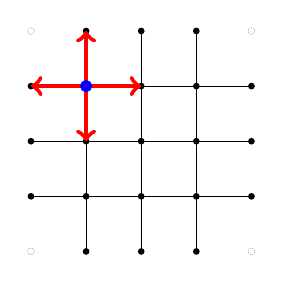
\begin{tikzpicture}[scale=0.7]
  \def\gridsize{1}
  \def\gridmarksize{0.1}
  \draw[step=\gridsize,black,thin] (0,0) grid (4,4);
  \draw[step=4*\gridsize,white,thin] (0,0) grid (4,4);
  \foreach \x in {0,1,...,4} {
      \foreach \y in {0,1,...,4} {
          \filldraw (\x,\y) circle (\gridmarksize/2);
      }
  }
  \foreach \x in {0,4} {
      \foreach \y in {0,4} {
          \filldraw[white] (\x,\y) circle (\gridmarksize/2);
      }
  }
  \foreach \x/\y in {1/3} {
      \draw[->, red, ultra thick] (\x,\y) -- (\x,\y+1); % 向上箭头
      \draw[->, red, ultra thick] (\x,\y) -- (\x+1,\y); % 向右箭头
      \draw[->, red, ultra thick] (\x,\y) -- (\x-1,\y); % 向左箭头
      \draw[->, red, ultra thick] (\x,\y) -- (\x,\y-1); % 向下箭头
  }
  \filldraw (1,3)[blue] circle (\gridmarksize);
  \end{tikzpicture}
\end{figure}

\subsubsection{Neumann 边值条件}\label{Neumann}

\[\boxed{\dpart{u}{\bm{n}}{} = g, \text{on~~} \partial \Omega}\]

本程序包采用延拓的方式来建立 Neumann 边值条件的差分格式,
对于所有 $(x_i, y_j), \quad i = 0, \dots, n, j = 0, \dots, n$ 分别建立和 \eqref{eq1} 
相同的五点差分方程,对于边界上的点,利用延拓点建立一个径向导数有限差分方程(以左边界为例):
\begin{equation}
  \dfrac{U_{-1, j} - U_{1, j}}{2} = g(x_0, y_j), j = 1, \dots, n-1
  \label{eq2}
\end{equation}
定义 $\UB = [U_{0, 0}, \dots, U_{n, n}, U_{-1, 1}, \dots, U_{-1, n-1}, U_{n+1, 1}, \dots, U_{n+1, n-1}, U_{1, -1}, \dots, U_{n-1, -1}, U_{1, n+1}, \dots, U_{n-1, n+1}]^T$,
根据 \eqref{eq1},\eqref{eq2},得到方程组 $A\UB = \FB$,\\其中 $\FB = [f(x_0, y_0), \cdots, f(x_n, y_n), g(x_{-1}, y_1), \dots, g(x_{-1}, y_{n-1}), g(x_{1}, y_{-1}), \dots, g(x_{n-1}, y_{-1}), g(x_{1}, y_{n+1}), \dots,$\\$g(x_{n-1}, y_{n+1})]^T$。
差分格式如下图所示:
% \newline
\begin{figure}[H]
  \centering
  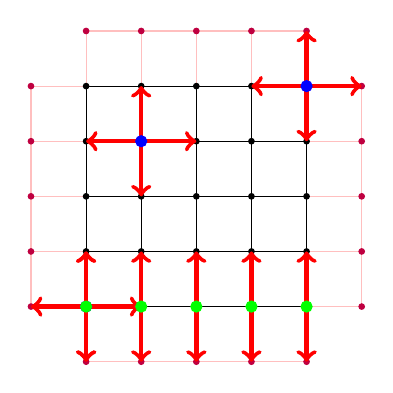
\begin{tikzpicture}[scale=0.7]
  \def\gridsize{1}
  \def\gridmarksize{0.1}
  \draw[step=\gridsize,pink,thin] (-1,0) grid (0,4);
  \draw[step=\gridsize,pink,thin] (4,0) grid (5,4);
  \draw[step=\gridsize,pink,thin] (0,4) grid (4,5);
  \draw[step=\gridsize,pink,thin] (0,-1) grid (4,0);
  \draw[step=\gridsize,black,thin] (0,0) grid (4,4);
  \foreach \x in {0,1,...,4} {
      \foreach \y in {0,1,...,4} {
          \filldraw (\x,\y) circle (\gridmarksize/2);
      }
  }
  \foreach \x in {0,...,4} {
      \foreach \y in {-1,5} {
          \filldraw (\x,\y)[purple] circle (\gridmarksize/2);
      }
  }
  \foreach \y in {0,...,4} {
      \foreach \x in {-1,5} {
          \filldraw (\x,\y)[purple] circle (\gridmarksize/2);
      }
  }
  \foreach \x/\y in {1/3, 4/4, 0/0} {
      \draw[->, red, ultra thick] (\x,\y) -- (\x,\y+1); % 向上箭头
      \draw[->, red, ultra thick] (\x,\y) -- (\x+1,\y); % 向右箭头
      \draw[->, red, ultra thick] (\x,\y) -- (\x-1,\y); % 向左箭头
      \draw[->, red, ultra thick] (\x,\y) -- (\x,\y-1); % 向下箭头
      \filldraw (\x, \y)[blue] circle (\gridmarksize);
  }
  \foreach \x/\y in {0/0, 1/0, 2/0, 3/0, 4/0} {
      \draw[->, red, ultra thick] (\x,\y) -- (\x,\y+1); % 向上箭头
      % \draw[->, red, thick] (\x,\y) -- (\x+1,\y); % 向右箭头
      % \draw[->, red, thick] (\x,\y) -- (\x-1,\y); % 向左箭头
      \draw[->, red, ultra thick] (\x,\y) -- (\x,\y-1); % 向下箭头
      \filldraw (\x, \y)[green] circle (\gridmarksize);
  }
  \end{tikzpicture}
\end{figure}

上述方程组具有 1 的自由度,为了消除矩阵的奇异性,我们选择强制增加条件 $U(0, 0) = 1$,并将该等式与第一个方程相加,
不规则区域的 Neumann 边值问题也做同样的处理。事实上,该部分可以修改为用户自定义的形式:用户给定
输入区域中某一点的值 $u(X_0)$,方程组中增加一个插值方程替换第一个方程,插值方法为取给定点附近的 6 个格点,
列出其关于给定点的 Taylor 展开是,求解系数满足 $\sum_{i = 1}^6 a_i U_{X_i} = u(X_0) + O(h^2)$,
处理方法与 \ref{ysnm} 类似。但我们认为这么做没有办法很好地展示 Neumann 边值问题“任意常数”的性质,
并且也增加了用户的使用复杂度,因此最后并没有实现。

\subsubsection{混合 边值条件}

本程序支持为规则区域的四条边界定义不同的边值条件,即可以部分为 Nuemann 边值条件,部分为 Dirichlet 边值条件。 
考虑 $(x_0, y_n), (x_n, y_n), (x_0, y_0), (x_n, y_0)$ 处的处理方式,
对于一个角 $P$,如果其相邻两条边均为 Neumann 边值条件,则采用与 \ref{Neumann} 类似的构造方法,在该点处分别建立
x,y 轴方向的径向导数方程和一个五点差分方程;若都是 Dirichlet 条件,与 \ref{Dirichlet} 类似,该点处不点不作为方程组未知数;
若一个是 Neumann 边值条件,一个是 Dirichlet 条件,则对于 Neumann 边值条件的方向,建立一个径向导数方程,
利用 Dirichlet 条件求出 $u(P) = g(P)$,建立方程 $U_P = g(P)$。

差分格式如下图所示(以左、下边界为 Nuemann 边值条件,右、上边界为 Dirichlet 边值条件为例):
\begin{figure}[H]
  \centering
  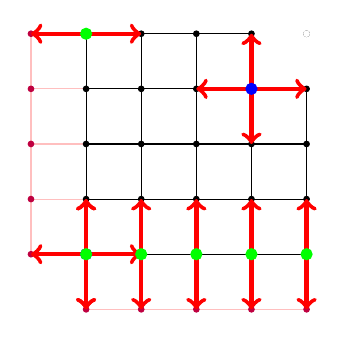
\begin{tikzpicture}[scale=0.7]
  \def\gridsize{1}
  \def\gridmarksize{0.1}
  \draw[step=\gridsize,pink,thin] (-1,0) grid (0,4);
  \draw[step=\gridsize,pink,thin] (0,-1) grid (4,0);
  \draw[step=\gridsize,black,thin] (0,0) grid (4,4);
  \draw[step=\gridsize,white,thin] (3,4) grid (4,4);
  \draw[step=\gridsize,white,thin] (4,3) grid (4,4);
  \foreach \x in {0,1,...,4} {
      \foreach \y in {0,1,...,4} {
          \filldraw (\x,\y) circle (\gridmarksize/2);
      }
  }
  \foreach \x in {0,...,4} {
      \foreach \y in {-1} {
          \filldraw (\x,\y)[purple] circle (\gridmarksize/2);
      }
  }
  \foreach \y in {0,...,4} {
      \foreach \x in {-1} {
          \filldraw (\x,\y)[purple] circle (\gridmarksize/2);
      }
  }
  \filldraw[white] (4,4) circle (\gridmarksize/2);
  \foreach \x/\y in {3/3, 0/0} {
      \draw[->, red, ultra thick] (\x,\y) -- (\x,\y+1); % 向上箭头
      \draw[->, red, ultra thick] (\x,\y) -- (\x+1,\y); % 向右箭头
      \draw[->, red, ultra thick] (\x,\y) -- (\x-1,\y); % 向左箭头
      \draw[->, red, ultra thick] (\x,\y) -- (\x,\y-1); % 向下箭头
      \filldraw (\x, \y)[blue] circle (\gridmarksize);
  }
  \foreach \x/\y in {0/0, 1/0, 2/0, 3/0, 4/0} {
      \draw[->, red, ultra thick] (\x,\y) -- (\x,\y+1); % 向上箭头
      % \draw[->, red, thick] (\x,\y) -- (\x+1,\y); % 向右箭头
      % \draw[->, red, thick] (\x,\y) -- (\x-1,\y); % 向左箭头
      \draw[->, red, ultra thick] (\x,\y) -- (\x,\y-1); % 向下箭头
      \filldraw (\x, \y)[green] circle (\gridmarksize);
  }
  \foreach \x/\y in {0/4} {
      % \draw[->, red, ultra thick] (\x,\y) -- (\x,\y+1); % 向上箭头
      \draw[->, red, ultra thick] (\x,\y) -- (\x+1,\y); % 向右箭头
      \draw[->, red, ultra thick] (\x,\y) -- (\x-1,\y); % 向左箭头
      % \draw[->, red, ultra thick] (\x,\y) -- (\x,\y-1); % 向下箭头
      \filldraw (\x, \y)[green] circle (\gridmarksize);
  }
  \end{tikzpicture}
\end{figure}

\subsection{不规则区域}

不规则区域与规则区域的差别在中间被挖去了一个圆形区域,
对于所有不在圆形区域内的格点,仍然与规则区域采用相同的规则建立求解方程组,
关于外边界上的边值条件处理方式也仍然与规则区域相同。

为了保证上述过程,不得不引入新的位于圆形区域内部的延拓格点(为了满足五点差分的格式),
而延拓的格点的点值也作为未知量加入到方程组中,因此需要新增方程来保证方程组的可解性。

\subsubsection{圆上 Dirichlet 条件}

\[\boxed{u = g, \text{on~~} \partial D:= \{(x, y) : (x - x_c)^2 + (y - y_c)^2 = R^2\}}\]

对于圆内的格点,我们可以找到与其相邻的圆与格线的交点,使用一次插值的方式估计该交点处的点值,
作为一个新的方程。

具体的,以格点为 $(x_i, y_j)$,交点为 $(x_i + \theta h, y_j), \theta \in (0, 1)$,为例子,
用 $(x_i, y_j)$ 和 $(x_{i+1}, y_j)$ 的点值来估计交点:

\begin{equation}
  \theta U_{i+1, j} + (1 - \theta) U_{i, j} = g(x_i + \theta h, y_j)
  \label{eq4}
\end{equation}

注意如果相邻交点恰也为格点,即上述 $\theta = 1$ 的情况,
此时应采用如下格式:

\[
  \frac12 U_{i+2, j} + \frac12 U_{i, j} = g(x_{i+1}, y_j)
\]

该方法如下图所示:

\begin{figure}[H]
  \centering
  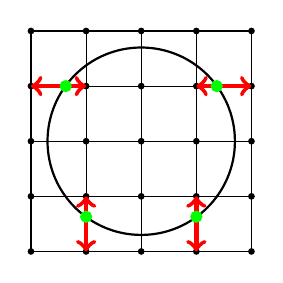
\begin{tikzpicture}[scale=0.7]
  \def\gridsize{1}
  \def\gridmarksize{0.1}
  \draw[step=\gridsize,black,thin] (0,0) grid (4,4);
  \foreach \x in {0,1,...,4} {
      \foreach \y in {0,1,...,4} {
          \filldraw (\x,\y) circle (\gridmarksize/2);
      }
  }
  \draw[thick] (2,2) circle (1.7);
  \foreach \x/\y in {1/0.63, 3/0.63} {
      \draw[->, red, ultra thick] (\x,\y) -- (\x,1); % 向上箭头
      \draw[->, red, ultra thick] (\x,\y) -- (\x,0); % 向下箭头
      \filldraw (\x, \y)[green] circle (\gridmarksize);
  }
  \foreach \x/\y in {0.63/3} {
      % \draw[->, red, ultra thick] (\x,\y) -- (\x,\y+1); % 向上箭头
      \draw[->, red, ultra thick] (\x,\y) -- (0,\y); % 向右箭头
      \draw[->, red, ultra thick] (\x,\y) -- (1,\y); % 向左箭头
      % \draw[->, red, ultra thick] (\x,\y) -- (\x,\y-1); % 向下箭头
      \filldraw (\x, \y)[green] circle (\gridmarksize);
  }
  \foreach \x/\y in {3.37/3} {
      % \draw[->, red, ultra thick] (\x,\y) -- (\x,\y+1); % 向上箭头
      \draw[->, red, ultra thick] (\x,\y) -- (3,\y); % 向右箭头
      \draw[->, red, ultra thick] (\x,\y) -- (4,\y); % 向左箭头
      % \draw[->, red, ultra thick] (\x,\y) -- (\x,\y-1); % 向下箭头
      \filldraw (\x, \y)[green] circle (\gridmarksize);
  }
  \end{tikzpicture}
\end{figure}

\subsubsection{圆上 Neumann 条件}\label{ysnm}

\[ \dpart{u}{\bm{n}}{} = g, \text{on~~} \partial D\]

对于圆内格点 $P$,作圆心 $C$ 到格点 $P$ 的射线,并交圆周于点 $Q(X_0, Y_0)$,
考虑用包括 $P$ 在内的 6 个格点(选取 $6$ 个是为了保证收敛阶为 2 阶),
作有限差分来表示 $Q$ 处的径向导数。

具体的,设 $\dpart{u}{\bm{n}}{} (Q) = u_x \cos \alpha + u_y \sin \alpha$,
设所取的附近 6 个格点的坐标分别为 $(X_i, Y_i), i = 1, \dots, 6$,
% 设 $(X_0, Y_0)$ 到 $(X_i, Y_i)$ 射线与x轴正方向夹角为 $\theta_i$,
则有
\begin{equation*}
\begin{aligned}
  u(X_i, Y_i) = &u(X_0, Y_0) + u_x\big|_{(X_0, Y_0)}(X_i - X_0) + u_y\big|_{(X_0, Y_0)}(Y_i - Y_0) +\frac12 u_{xx}\big|_{(X_0, Y_0)} (X_i - X_0)^2 \\
                &+ \frac12 u_{yy}\big|_{(X_0, Y_0)} (Y_i - Y_0)^2 + u_{xy}\big|_{(X_0, Y_0)} (X_i - X_0)(Y_i - Y_0) + O(h^3)
\end{aligned}
\end{equation*}
设
\[
  \dpart{u}{\bm{n}}{} (Q) = \sum_{i = 1}^6 a_i u(x_i, y_i) + O(h^2)
\]
为了保证上述方程组可解,需要保证 $X_1, \dots X_6$, $Y_1, \dots, Y_6$ 各有至少 3 个不同的值,

解得 $a_1, \dots, a_6$ 后,即得新增方程:
\[
\sum_{i = 1}^6 a_i U(X_i, Y_i) = g(X_0, Y_0)
\label{eq3}
\]
则有
\[
  \begin{bmatrix}
    1 & 1 & \cdots & 1 & 1 \\
    (X_1 - X_0) & (X_2 - X_0) & \cdots & (X_5 - X_0) & (X_6 - X_0) \\
    (Y_1 - Y_0) & (Y_2 - Y_0) & \cdots & (Y_5 - Y_0) & (Y_6 - Y_0) \\
    \frac12 (X_1 - X_0)^2 & \frac12 (X_2 - X_0)^2 & \cdots & \frac12 (X_5 - X_0)^2 & \frac12 (X_6 - X_0)^2 \\
    \frac12 (Y_1 - Y_0)^2 & \frac12 (Y_2 - Y_0)^2 & \cdots & \frac12 (Y_5 - Y_0)^2 & \frac12 (Y_6 - Y_0)^2 \\
    (X_1 - X_0)(Y_1 - Y_0) & (X_2 - X_0)(Y_2 - Y_0) & \cdots & (X_5 - X_0)(Y_5 - Y_0) & (X_6 - X_0)(Y_6 - Y_0)
  \end{bmatrix}
  \begin{bmatrix}
    a_1 \\ a_2 \\ a_3 \\ a_4 \\ a_5 \\ a_6
  \end{bmatrix}
  =
  \begin{bmatrix}
    0 \\ \cos \alpha \\ \sin \alpha \\ 0 \\ 0 \\ 0 
  \end{bmatrix}
\]

该方法如下图所示:

\begin{figure}[H]
  \centering
  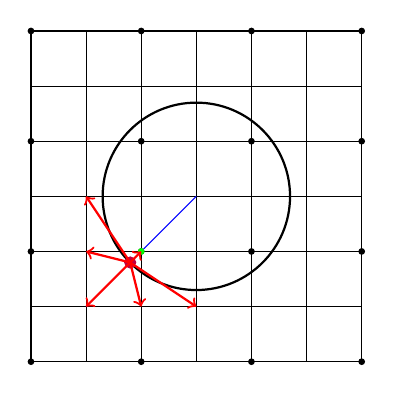
\begin{tikzpicture}[scale=0.7]
  \def\gridsize{1}
  \def\gridmarksize{0.1}
  \draw[step=\gridsize,black,thin] (-1,-1) grid (5,5);
  \foreach \x in {-1,1,...,5} {
      \foreach \y in {-1,1,...,5} {
          \filldraw (\x,\y) circle (\gridmarksize/2);
      }
  }
  \draw[thick] (2,2) circle (1.7);
  \draw[blue, thin] (0,0) -- (2,2);
  \filldraw (0.8, 0.8)[purple] circle (\gridmarksize);
  \filldraw (1, 1)[green] circle (\gridmarksize/2);
  \foreach \x/\y in {1/0.63} {
      \draw[->, red, thick] (0.8,0.8) -- (1,1); 
      \draw[->, red, thick] (0.8,0.8) -- (0,1); 
      \draw[->, red, thick] (0.8,0.8) -- (1,0); 
      \draw[->, red, thick] (0.8,0.8) -- (0,0); 
      \draw[->, red, thick] (0.8,0.8) -- (0,2); 
      \draw[->, red, thick] (0.8,0.8) -- (2,0);
  }
  \end{tikzpicture}
\end{figure}

我们至少需要保证圆周在每个方向距离 $\Omega$ 的外边界至少有 $2$ 个以上的格点。
否则,程序包将采用\textbf{另一种}方法(方法二)来解决这类的非规则区域 Neumann 边值条件问题,该方法
将圆周与格线的交点作为未知量加入方程:对于每个交点建立与 \eqref{eq3} 类似的方程,
其中 $6$ 个格点中有一个点为交点本身;对于圆周内的延拓格点,找到与其相邻的圆与格线的交点,
使用一次插值得到方程,我们可将 \eqref{eq4} 改造如下:
\begin{equation}
  \theta U_{i+1, j} + (1 - \theta) U_{i,j} = U(x_i + \theta h, y_j)
\end{equation}
该方法虽然理论收敛阶也为2,但是求解的效果远远不如原方法,事实上,
只需要加细网格就可以避免无法满足原方法条件的情况。如果不得不使用方法二来求解问题,
程序将给出警告:

\begin{lstlisting}
[warning]the circle is too near to the border, we may use another method to solve your problem
\end{lstlisting}

% \subsection{收敛性证明}


\section{样例测试及结果}

该部分说明此程序包在样例测试中的求解表现。

\subsection{测试说明}

本程序包对于三个 Poisson 方程关于不同的边值条件提供了若干测试数据,
测试数据位于目录 \texttt{/data} 下。

在根目录下编译并求解所有样例:
\begin{lstlisting}
  make all # compile
  make run
\end{lstlisting}

该指令将会编译 \texttt{/test.cpp},并且调用 \texttt{test} 按照字典序依次
运行所有的样例(\texttt{/data} 下的所有 JSON 文件),并且保存样例的误差分析结果至 \texttt{/res/test\_analysis.txt}。
测试输出(离散网格点值的求解结果)将会以表格的形式保存至 \texttt{/res/<Input File Name>.csv}。

对测试输出进行绘图:
\begin{lstlisting}
  make plot
\end{lstlisting}

该指令将会对保存在 \texttt{/res/} 目录下的所有 csv 输出文件进行绘图,
并且将结果保存在 \texttt{/res/} 下,命名与原文件相同,类型为 png。

测试点一共有 $6 \times 5 \times 3 = 90$ 个,所以测试耗时比较长( \texttt{Grid\_n = 128} 的测试样例平均需要运行
 1 分钟以上 ),
因此程序包提供了一份测试结果的备份,位于 \texttt{/res\_bac} 目录,
便于用户直接查看。

\subsection{测试样例1}

\[
  u(x, y) = \exp (y + \sin x), \Omega = [0, 1]^2
\]

\subsubsection{规则区域}

\subsubsubsection{Dirichlet 边值条件}

\[
  \begin{cases}
    - \Delta u = -(1 - \sin x + \cos^2 x) \exp(\sin x + y), \text{in~~} \Omega \\
    u = \exp(\sin x + y), \text{on~~} \partial \Omega 
  \end{cases}
\]

求解结果如下图:

\begin{figure}[H]
  \centering
  \begin{subfigure}[b]{0.18\textwidth}
      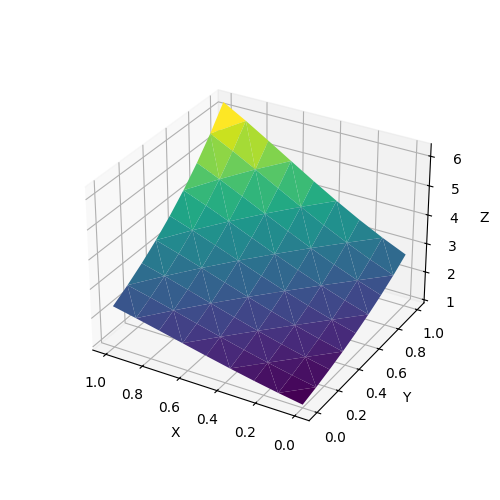
\includegraphics[width=\textwidth]{../../res_bac/res-[data|1-Dirichlet-regular-a8].png}
      \caption{$n =  8$}
  \end{subfigure}
  \hfill
  \begin{subfigure}[b]{0.18\textwidth}
      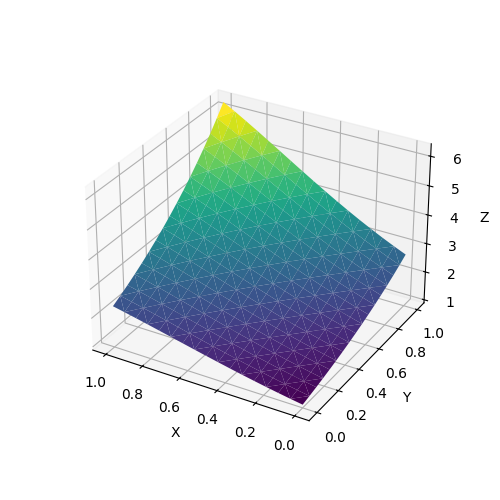
\includegraphics[width=\textwidth]{../../res_bac/res-[data|1-Dirichlet-regular-b16].png}
      \caption{$n= 16$}
  \end{subfigure}
  \hfill
  \begin{subfigure}[b]{0.18\textwidth}
      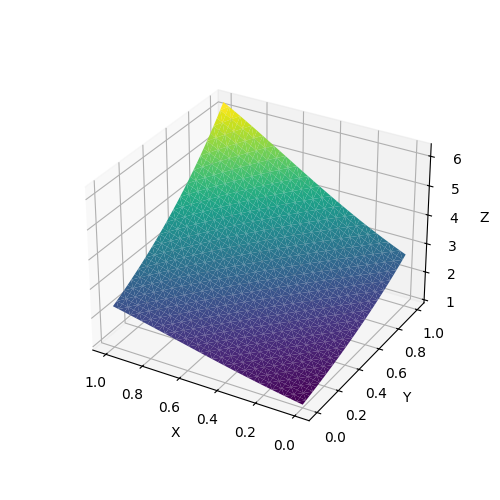
\includegraphics[width=\textwidth]{../../res_bac/res-[data|1-Dirichlet-regular-c32].png}
      \caption{$n = 32$}
  \end{subfigure}
  \hfill
  \begin{subfigure}[b]{0.18\textwidth}
      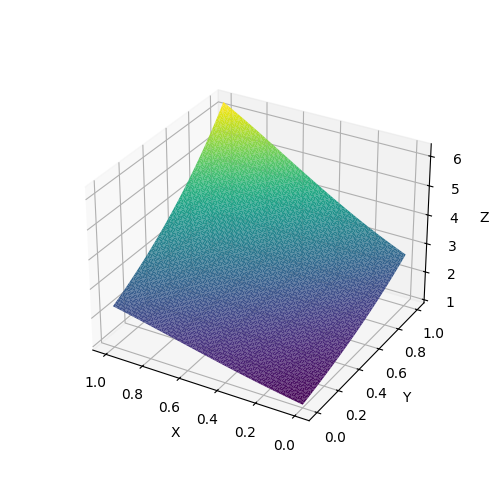
\includegraphics[width=\textwidth]{../../res_bac/res-[data|1-Dirichlet-regular-d64].png}
      \caption{$n = 64$}
  \end{subfigure}
  \hfill
  \begin{subfigure}[b]{0.18\textwidth}
      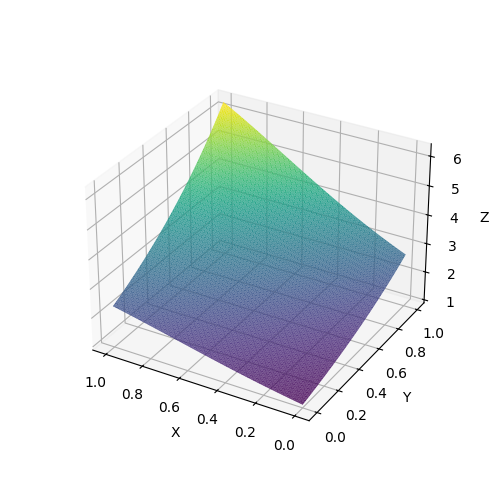
\includegraphics[width=\textwidth]{../../res_bac/res-[data|1-Dirichlet-regular-e128].png}
      \caption{$n = 128$}
  \end{subfigure}
\end{figure}

误差分析如下表:

\begin{table}[H]
  \centering
  \begin{tabular}{|c|c|c|c|c|c|c|}
  \hline
   & 8 & 16 & 32 & 64 & 128 & convergence rate \\
  \hline
  Norm-1 & 1.8732e-04 & 5.1981e-05 & 1.3745e-05 & 3.5391e-06 & 8.9830e-07 & 1.978 \\
  Norm-2 & 2.5898e-04 & 6.7615e-05 & 1.7346e-05 & 4.3983e-06 & 1.1078e-06 & 1.989 \\
  Norm-$\infty$ & 5.3698e-04 & 1.3760e-04 & 3.4450e-05 & 8.6241e-06 & 2.1565e-06 & 2.000 \\
  \hline
  \end{tabular}
  \end{table}

\subsubsubsection{Neumann 边值条件}

\[
  \begin{cases}
    - \Delta u = -(1 - \sin x + \cos^2 x) \exp(\sin x + y), \text{in~~} \Omega \\
    \apart{u}{\bm{n}}{} = -\exp(\sin x), y = 0 \\
    \apart{u}{\bm{n}}{} = -\exp(y), x = 0 \\
    \apart{u}{\bm{n}}{} = \cos 1 \cdot \exp(\sin 1 + y), x = 1 \\ 
    \apart{u}{\bm{n}}{} = \exp(\sin x + 1), y = 1
  \end{cases}
\]

求解结果如下图:

\begin{figure}[H]
  \centering
  \begin{subfigure}[b]{0.18\textwidth}
      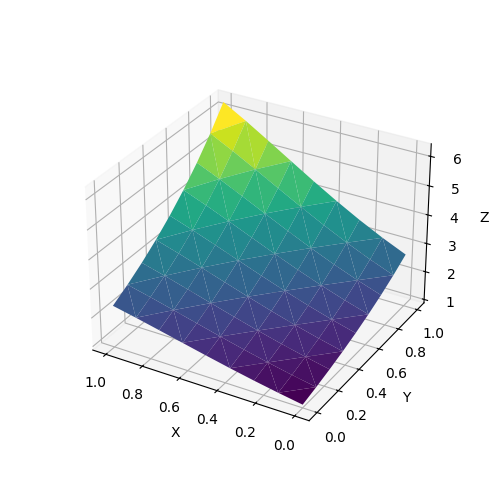
\includegraphics[width=\textwidth]{../../res_bac/res-[data|1-Neumann-regular-a8].png}
      \caption{$n =  8$}
  \end{subfigure}
  \hfill
  \begin{subfigure}[b]{0.18\textwidth}
      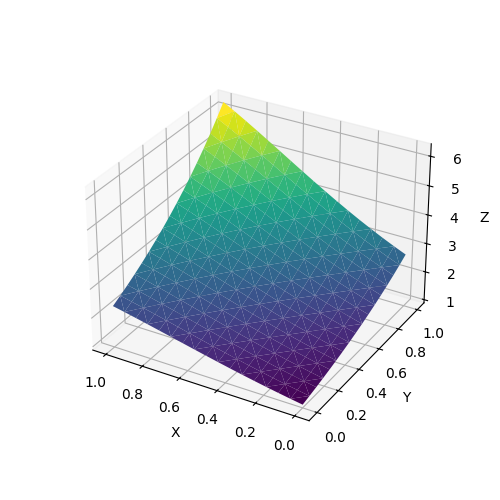
\includegraphics[width=\textwidth]{../../res_bac/res-[data|1-Neumann-regular-b16].png}
      \caption{$n= 16$}
  \end{subfigure}
  \hfill
  \begin{subfigure}[b]{0.18\textwidth}
      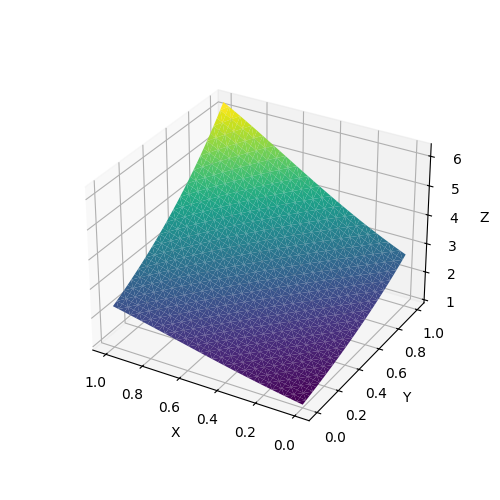
\includegraphics[width=\textwidth]{../../res_bac/res-[data|1-Neumann-regular-c32].png}
      \caption{$n = 32$}
  \end{subfigure}
  \hfill
  \begin{subfigure}[b]{0.18\textwidth}
      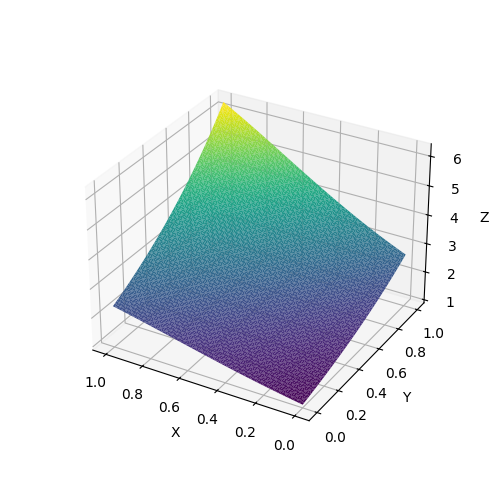
\includegraphics[width=\textwidth]{../../res_bac/res-[data|1-Neumann-regular-d64].png}
      \caption{$n = 64$}
  \end{subfigure}
  \hfill
  \begin{subfigure}[b]{0.18\textwidth}
      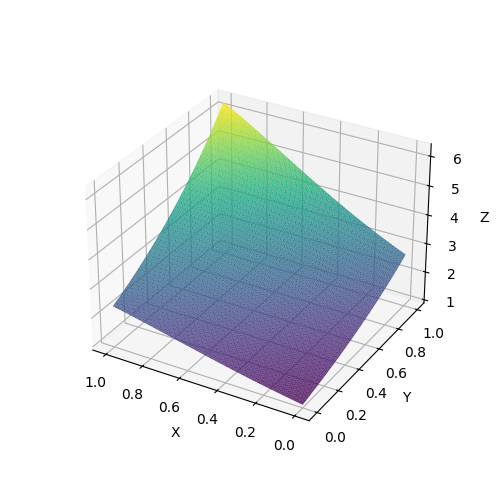
\includegraphics[width=\textwidth]{../../res_bac/res-[data|1-Neumann-regular-e128].png}
      \caption{$n = 128$}
  \end{subfigure}
\end{figure}

误差分析如下表:

\begin{table}[H]
  \centering
  \begin{tabular}{|c|c|c|c|c|c|c|}
  \hline
   & 8 & 16 & 32 & 64 & 128 & convergence rate \\
  \hline
  Norm-1 & 3.5392e-03 & 8.5950e-04 & 2.1038e-04 & 5.1896e-05 & 1.2876e-05 & 2.011 \\
  Norm-2 & 4.0957e-03 & 9.9946e-04 & 2.4517e-04 & 6.0525e-05 & 1.5018e-05 & 2.011 \\
  Norm-$\infty$ & 8.1409e-03 & 2.0968e-03 & 6.4677e-04 & 1.9814e-04 & 5.8749e-05 & 1.754 \\
  \hline
  \end{tabular}
  \end{table}

\subsubsubsection{混合边值条件}

\[
  \begin{cases}
    - \Delta u = -(1 - \sin x + \cos^2 x) \exp(\sin x + y), \text{in~~} \Omega \\
    u = \exp(\sin x + y), y = 0 \\
    u= \exp(\sin x + y), x = 0 \\
    \apart{u}{\bm{n}}{} = \cos 1 \cdot \exp(\sin 1 + y), x = 1 \\
    \apart{u}{\bm{n}}{} = \exp(\sin x + 1), y = 1
  \end{cases}
\]

求解结果如下图:

\begin{figure}[H]
  \centering
  \begin{subfigure}[b]{0.18\textwidth}
      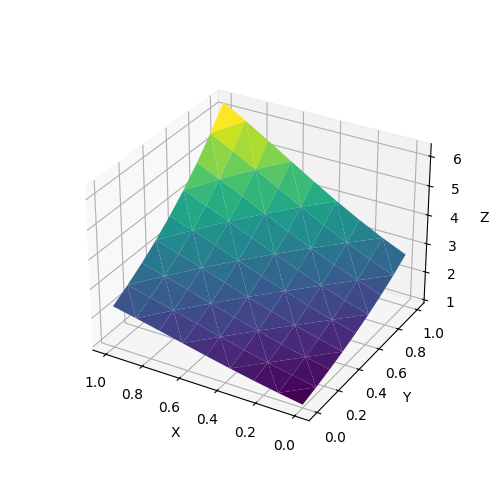
\includegraphics[width=\textwidth]{../../res_bac/res-[data|1-mixed-regular-a8].png}
      \caption{$n =  8$}
  \end{subfigure}
  \hfill
  \begin{subfigure}[b]{0.18\textwidth}
      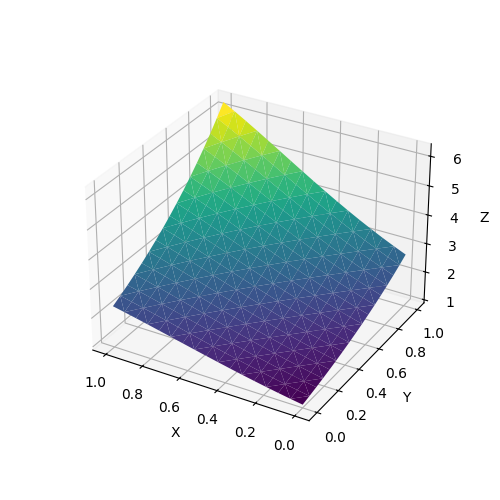
\includegraphics[width=\textwidth]{../../res_bac/res-[data|1-mixed-regular-b16].png}
      \caption{$n= 16$}
  \end{subfigure}
  \hfill
  \begin{subfigure}[b]{0.18\textwidth}
      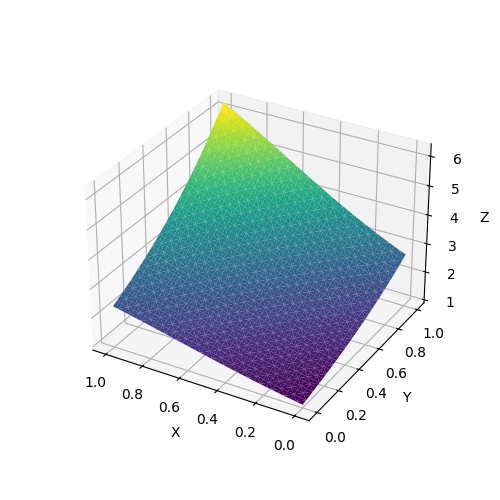
\includegraphics[width=\textwidth]{../../res_bac/res-[data|1-mixed-regular-c32].png}
      \caption{$n = 32$}
  \end{subfigure}
  \hfill
  \begin{subfigure}[b]{0.18\textwidth}
      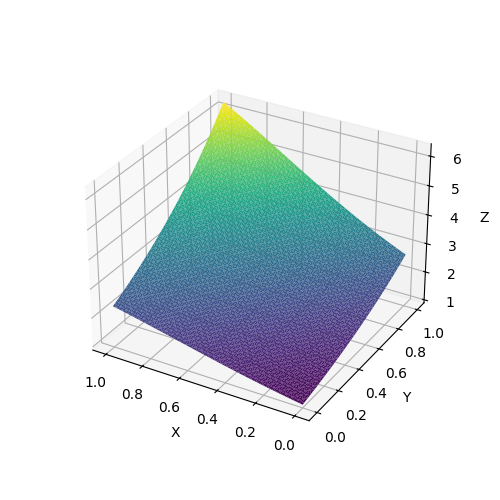
\includegraphics[width=\textwidth]{../../res_bac/res-[data|1-mixed-regular-d64].png}
      \caption{$n = 64$}
  \end{subfigure}
  \hfill
  \begin{subfigure}[b]{0.18\textwidth}
      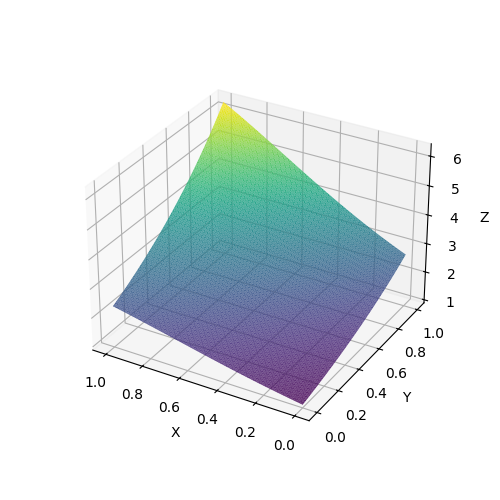
\includegraphics[width=\textwidth]{../../res_bac/res-[data|1-mixed-regular-e128].png}
      \caption{$n = 128$}
  \end{subfigure}
\end{figure}

误差分析如下表:

\begin{table}[H]
  \centering
  \begin{tabular}{|c|c|c|c|c|c|c|}
  \hline
   & 8 & 16 & 32 & 64 & 128 & convergence rate \\
  \hline
  Norm-1 & 1.4173e-03 & 3.4119e-04 & 8.3505e-05 & 2.0646e-05 & 5.1317e-06 & 2.008 \\
  Norm-2 & 2.2667e-03 & 5.3570e-04 & 1.2977e-04 & 3.1898e-05 & 7.9046e-06 & 2.013 \\
  Norm-$\infty$ & 6.7443e-03 & 1.6985e-03 & 4.2452e-04 & 1.0612e-04 & 2.6530e-05 & 2.000  \\
  \hline
  \end{tabular}
  \end{table}

\subsubsection{不规则区域}

\subsubsubsection{Dirichlet 边值条件}

取 $D = {(x, y) : (x - 0.5)^2 + (y - 0.5)^2 \le 0.2^2}$

\[
  \begin{cases}
    - \Delta u = -(1 - \sin x + \cos^2 x) \exp(\sin x + y), \text{in~~} \Omega \fxg D \\
    u = \exp(\sin x + y), \text{on~~} \partial \Omega \fxg D \\
  \end{cases}
\]

求解结果如下图:

\begin{figure}[H]
  \centering
  \begin{subfigure}[b]{0.18\textwidth}
      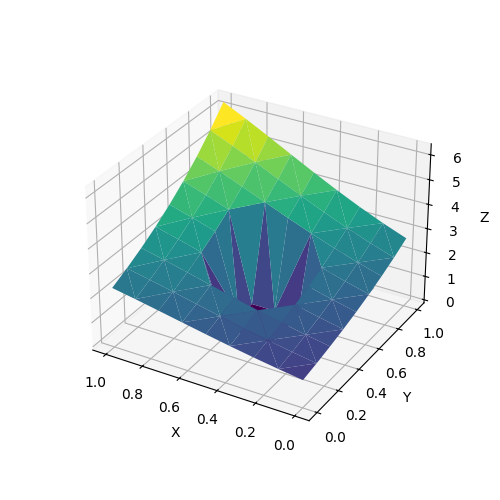
\includegraphics[width=\textwidth]{../../res_bac/res-[data|1-Dirichlet-irregular-a8].png}
      \caption{$n =  8$}
  \end{subfigure}
  \hfill
  \begin{subfigure}[b]{0.18\textwidth}
      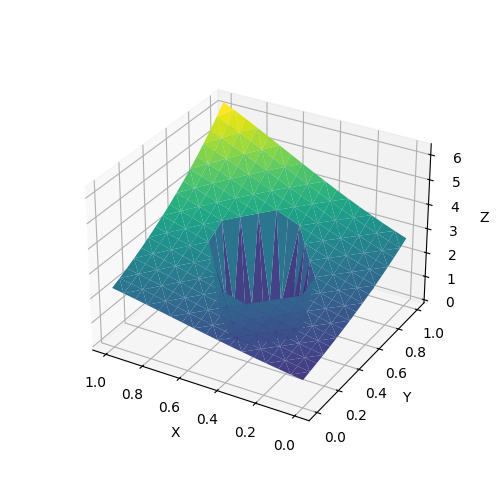
\includegraphics[width=\textwidth]{../../res_bac/res-[data|1-Dirichlet-irregular-b16].png}
      \caption{$n= 16$}
  \end{subfigure}
  \hfill
  \begin{subfigure}[b]{0.18\textwidth}
      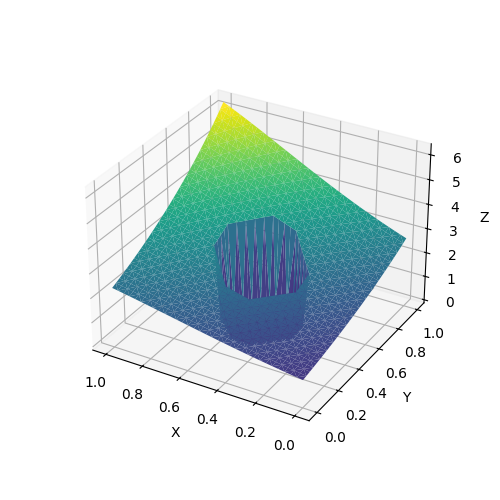
\includegraphics[width=\textwidth]{../../res_bac/res-[data|1-Dirichlet-irregular-c32].png}
      \caption{$n = 32$}
  \end{subfigure}
  \hfill
  \begin{subfigure}[b]{0.18\textwidth}
      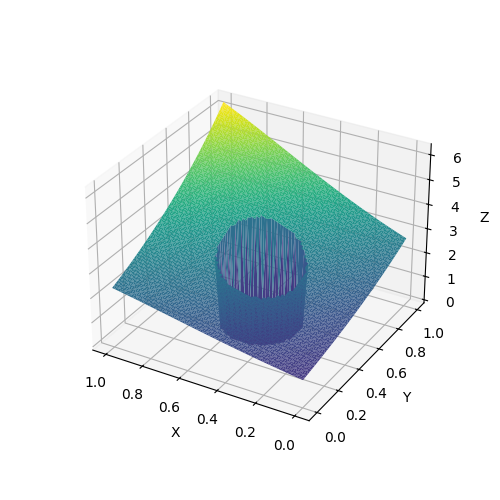
\includegraphics[width=\textwidth]{../../res_bac/res-[data|1-Dirichlet-irregular-d64].png}
      \caption{$n = 64$}
  \end{subfigure}
  \hfill
  \begin{subfigure}[b]{0.18\textwidth}
      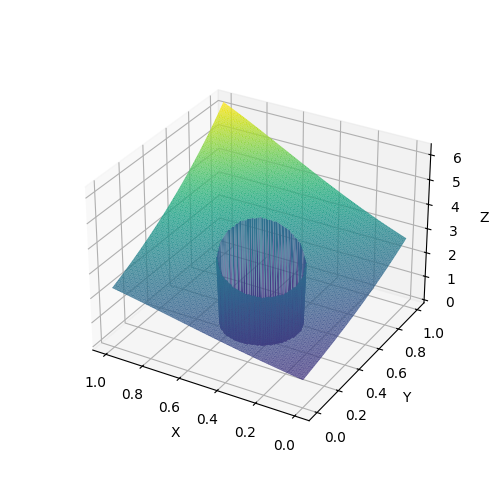
\includegraphics[width=\textwidth]{../../res_bac/res-[data|1-Dirichlet-irregular-e128].png}
      \caption{$n = 128$}
  \end{subfigure}
  \caption{Images of matrices}\label{fig:matrices}
\end{figure}

误差分析如下表:

\begin{table}[H]
  \centering
  \begin{tabular}{|c|c|c|c|c|c|c|}
  \hline
   & 8 & 16 & 32 & 64 & 128 & convergence rate \\
  \hline
  Norm-1 & 4.8348e-04 & 7.7600e-05 & 2.5512e-05 & 8.0168e-06 & 2.0462e-06 & 1.970 \\
  Norm-2 & 8.6250e-04 & 1.2588e-04 & 4.2190e-05 & 1.2788e-05 & 3.1676e-06 & 2.012 \\
  Norm-$\infty$ & 3.6669e-03 & 5.1496e-04 & 2.8639e-04 & 8.1283e-05 & 2.3051e-05 & 1.818 \\
  \hline
  \end{tabular}
\end{table}


\subsubsubsection{Neumann 边值条件}

取 $D = {(x, y) : (x - 0.52)^2 + (y - 0.52)^2 \le 0.21^2}$

\[
  \begin{cases}
    - \Delta u = -(1 - \sin x + \cos^2 x) \exp(\sin x + y), \text{in~~} \Omega\fxg D \\
    \apart{u}{\bm{n}}{} = -\exp(\sin x), y = 0 \\
    \apart{u}{\bm{n}}{} = -\exp(y), x = 0 \\
    \apart{u}{\bm{n}}{} = \cos 1 \cdot \exp(\sin 1 + y), x = 1 \\ 
    \apart{u}{\bm{n}}{} = \exp(\sin x + 1), y = 1 \\
    \apart{u}{\bm{n}}{} = \cos x \cdot \exp(\sin x + y) \cdot (x - 0.52)/0.21 + \exp(\sin x + y) \cdot (y - 0.52) / 0.21, \text{on~~} \partial D
  \end{cases}
\]

求解结果如下图:

\begin{figure}[H]
  \centering
  \begin{subfigure}[b]{0.18\textwidth}
      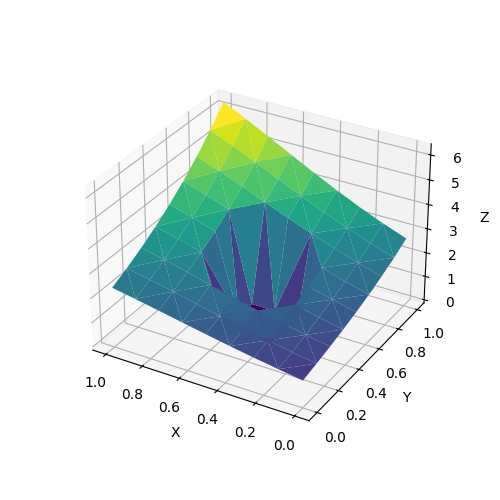
\includegraphics[width=\textwidth]{../../res_bac/res-[data|1-Neumann-irregular-a8].png}
      \caption{$n =  8$}
  \end{subfigure}
  \hfill
  \begin{subfigure}[b]{0.18\textwidth}
      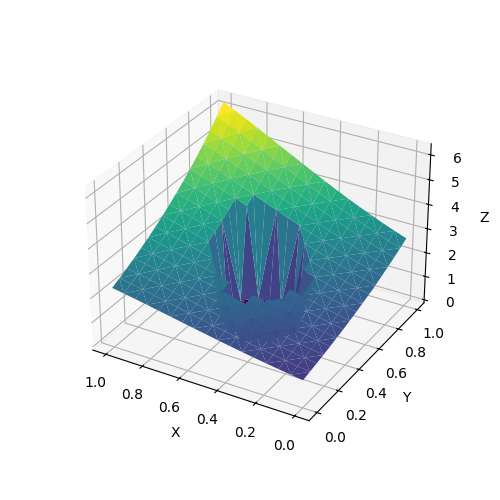
\includegraphics[width=\textwidth]{../../res_bac/res-[data|1-Neumann-irregular-b16].png}
      \caption{$n= 16$}
  \end{subfigure}
  \hfill
  \begin{subfigure}[b]{0.18\textwidth}
      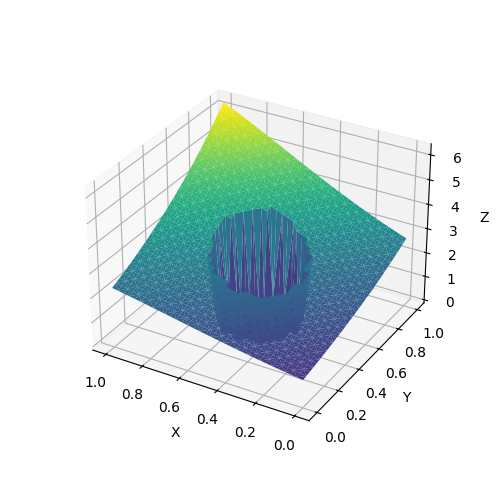
\includegraphics[width=\textwidth]{../../res_bac/res-[data|1-Neumann-irregular-c32].png}
      \caption{$n = 32$}
  \end{subfigure}
  \hfill
  \begin{subfigure}[b]{0.18\textwidth}
      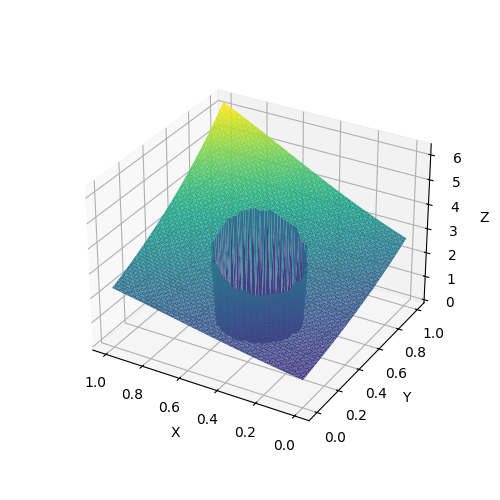
\includegraphics[width=\textwidth]{../../res_bac/res-[data|1-Neumann-irregular-d64].png}
      \caption{$n = 64$}
  \end{subfigure}
  \hfill
  \begin{subfigure}[b]{0.18\textwidth}
      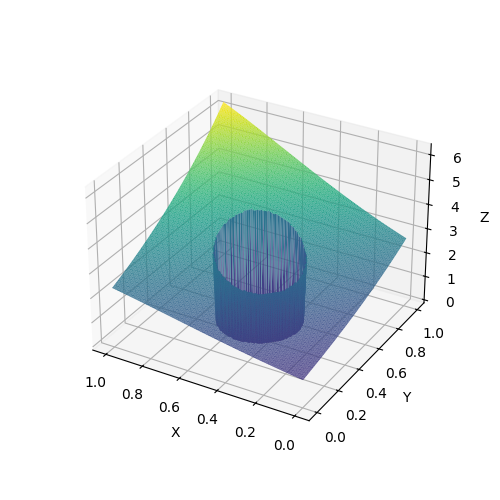
\includegraphics[width=\textwidth]{../../res_bac/res-[data|1-Neumann-irregular-e128].png}
      \caption{$n = 128$}
  \end{subfigure}
\end{figure}

误差分析如下表:

\begin{table}[H]
  \centering
  \begin{tabular}{|c|c|c|c|c|c|c|}
  \hline
   & 8 & 16 & 32 & 64 & 128 & convergence rate \\
  \hline
  Norm-1 & 4.8601e-03 & 1.1380e-03 & 2.4802e-04 & 6.1841e-05 & 1.5454e-05 & 2.000 \\
  Norm-2 & 5.4052e-03 & 1.2953e-03 & 2.8044e-04 & 6.9584e-05 & 1.7363e-05 & 2.003 \\
  Norm-$\infty$ & 9.3239e-03 & 3.6538e-03 & 8.1236e-04 & 2.2576e-04 & 5.2197e-05 & 2.113 \\
  \hline
  \end{tabular}
  \end{table}

\subsubsubsection{混合边值条件}

取 $D = {(x, y) : (x - 0.5)^2 + (y - 0.6)^2 \le 0.2^2}$

\[
  \begin{cases}
    - \Delta u = -(1 - \sin x + \cos^2 x) \exp(\sin x + y), \text{in~~} \Omega \fxg D \\
    u = \exp(\sin x + y), {on~~} \partial \Omega \\
    \apart{u}{\bm{n}}{} = \cos x \cdot \exp(\sin x + y) \cdot (x - 0.5)/0.2 + \exp(\sin x + y) \cdot (y - 0.6) / 0.2, \text{on~~} \partial D
  \end{cases}
\]

求解结果如下图:

\begin{figure}[H]
  \centering
  \begin{subfigure}[b]{0.18\textwidth}
      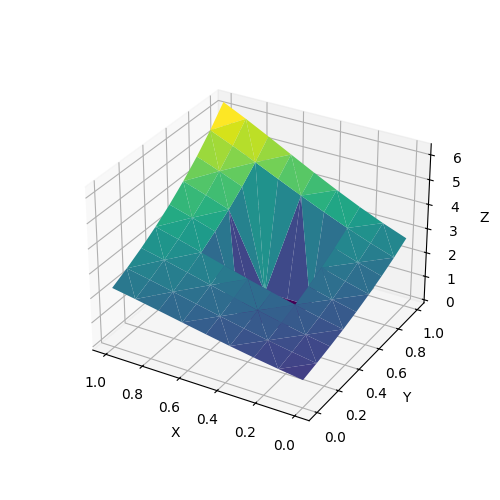
\includegraphics[width=\textwidth]{../../res_bac/res-[data|1-mixed-irregular-a8].png}
      \caption{$n =  8$}
  \end{subfigure}
  \hfill
  \begin{subfigure}[b]{0.18\textwidth}
      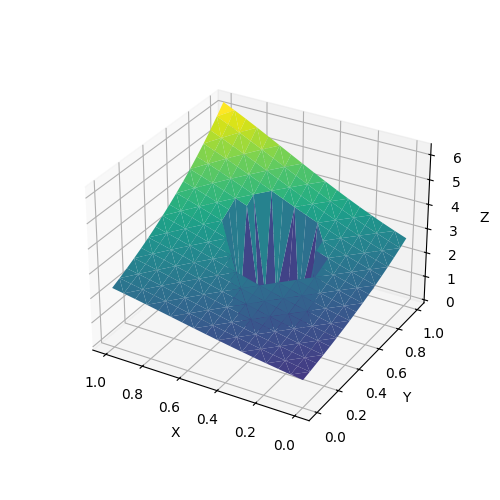
\includegraphics[width=\textwidth]{../../res_bac/res-[data|1-mixed-irregular-b16].png}
      \caption{$n= 16$}
  \end{subfigure}
  \hfill
  \begin{subfigure}[b]{0.18\textwidth}
      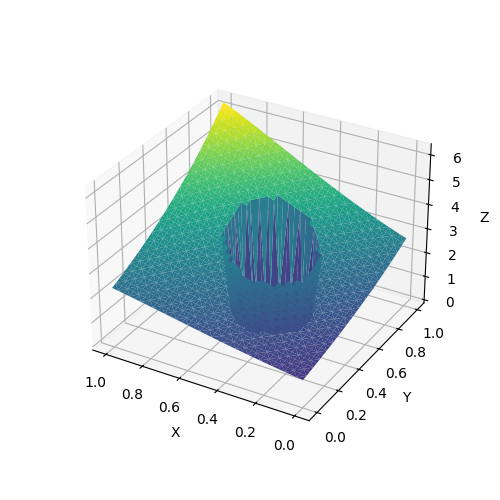
\includegraphics[width=\textwidth]{../../res_bac/res-[data|1-mixed-irregular-c32].png}
      \caption{$n = 32$}
  \end{subfigure}
  \hfill
  \begin{subfigure}[b]{0.18\textwidth}
      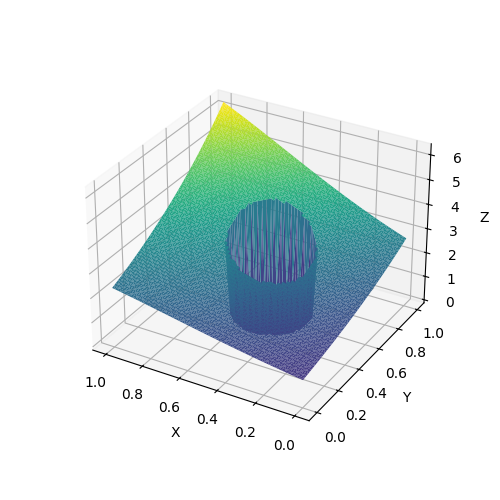
\includegraphics[width=\textwidth]{../../res_bac/res-[data|1-mixed-irregular-d64].png}
      \caption{$n = 64$}
  \end{subfigure}
  \hfill
  \begin{subfigure}[b]{0.18\textwidth}
      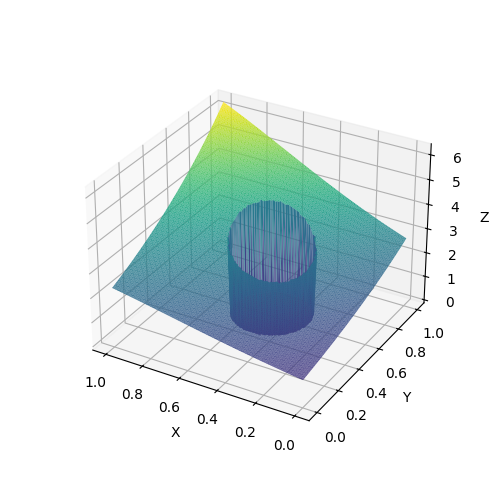
\includegraphics[width=\textwidth]{../../res_bac/res-[data|1-mixed-irregular-e128].png}
      \caption{$n = 128$}
  \end{subfigure}
\end{figure}

误差分析如下表:

\begin{table}[H]
  \centering
  \begin{tabular}{|c|c|c|c|c|c|c|}
  \hline
   & 8 & 16 & 32 & 64 & 128 & convergence rate \\
  \hline
  Norm-1 & 9.3127e-04 & 9.1094e-05 & 2.0532e-05 & 5.7256e-06 & 1.3168e-06 & 2.120 \\
  Norm-2 & 1.6941e-03 & 1.4884e-04 & 3.1919e-05 & 8.9742e-06 & 2.0896e-06 & 2.102 \\
  Norm-$\infty$ & 6.8751e-03 & 5.9106e-04 & 1.3182e-04 & 3.9069e-05 & 9.8320e-06 & 1.990 \\
  \hline
  \end{tabular}
  \end{table}

\subsection{测试样例2}

\[
  u(x, y) = \sin x \cos y, \Omega = [0, 1]^2
\]


\subsubsection{规则区域}

\subsubsubsection{Dirichlet 边值条件}

\[
\begin{cases}
  - \Delta u = 2\sin x \cos y, \text{in~~} \Omega \\
  u = \sin x \cos y, \text{on ~~} \partial \Omega
\end{cases}
\]

求解结果如下图:

\begin{figure}[H]
  \centering
  \begin{subfigure}[b]{0.18\textwidth}
      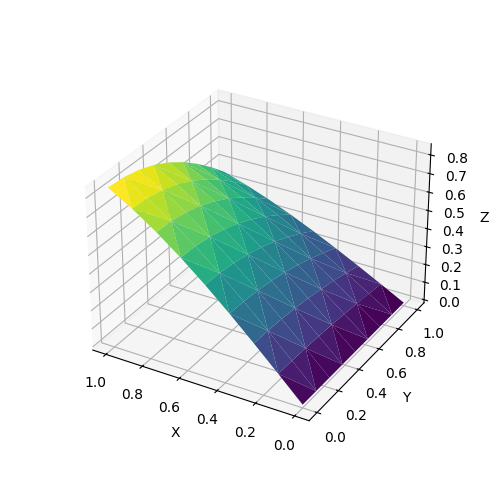
\includegraphics[width=\textwidth]{../../res_bac/res-[data|2-Dirichlet-regular-a8].png}
      \caption{$n =  8$}
  \end{subfigure}
  \hfill
  \begin{subfigure}[b]{0.18\textwidth}
      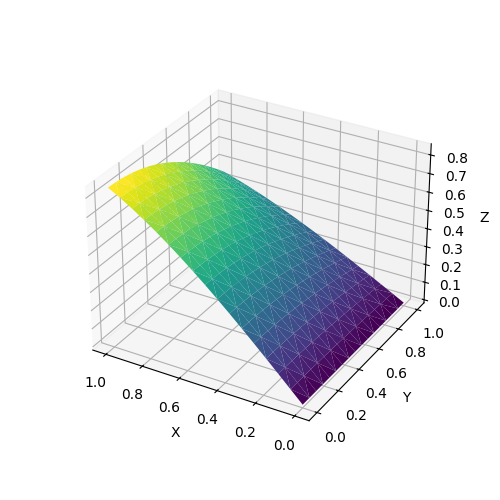
\includegraphics[width=\textwidth]{../../res_bac/res-[data|2-Dirichlet-regular-b16].png}
      \caption{$n= 16$}
  \end{subfigure}
  \hfill
  \begin{subfigure}[b]{0.18\textwidth}
      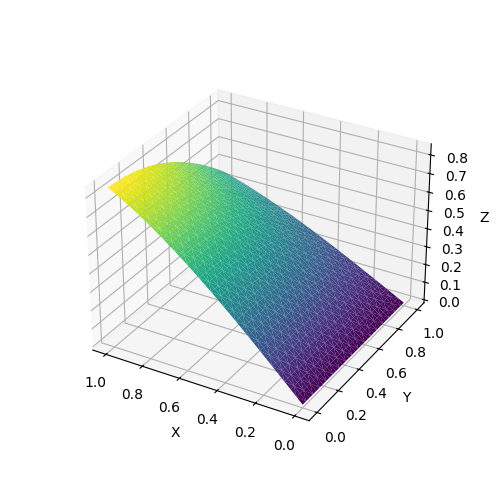
\includegraphics[width=\textwidth]{../../res_bac/res-[data|2-Dirichlet-regular-c32].png}
      \caption{$n = 32$}
  \end{subfigure}
  \hfill
  \begin{subfigure}[b]{0.18\textwidth}
      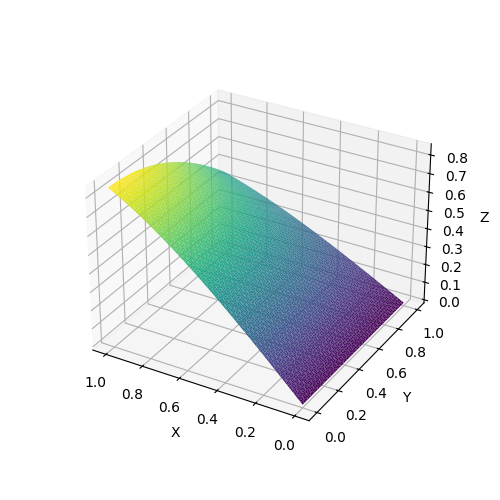
\includegraphics[width=\textwidth]{../../res_bac/res-[data|2-Dirichlet-regular-d64].png}
      \caption{$n = 64$}
  \end{subfigure}
  \hfill
  \begin{subfigure}[b]{0.18\textwidth}
      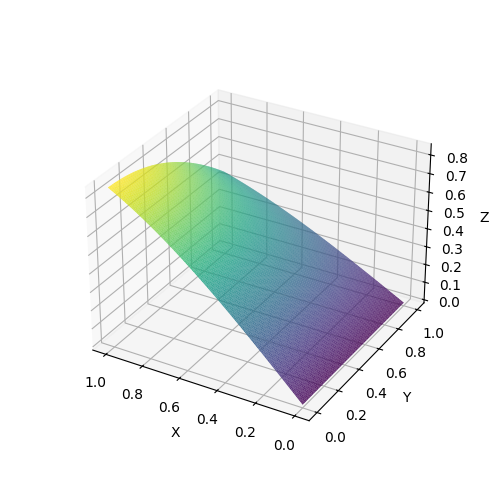
\includegraphics[width=\textwidth]{../../res_bac/res-[data|2-Dirichlet-regular-e128].png}
      \caption{$n = 128$}
  \end{subfigure}
\end{figure}

误差分析如下表:

\begin{table}[H]
  \centering
  \begin{tabular}{|c|c|c|c|c|c|c|}
  \hline
   & 8 & 16 & 32 & 64 & 128 & convergence rate \\
  \hline
  Norm-1 & 2.8971e-05 & 8.1076e-06 & 2.1486e-06 & 5.5350e-07 & 1.4050e-07 & 1.978 \\
  Norm-2 & 3.9556e-05 & 1.0371e-05 & 2.6633e-06 & 6.7550e-07 & 1.7010e-07 & 1.990 \\
  Norm-$\infty$ & 8.1105e-05 & 2.0543e-05 & 5.1505e-06 & 1.2896e-06 & 3.2240e-07 & 2.000 \\
  \hline
  \end{tabular}
  \end{table}

\subsubsubsection{Neumann 边值条件}

\[
\begin{cases}
  - \Delta u = 2\sin x \cos y, \text{in~~} \Omega \\
  \apart{u}{\bm{n}}{} = - \cos x \cos y, x = 0 \\
  \apart{u}{\bm{n}}{} = \cos x \cos y, x = 1 \\  
  \apart{u}{\bm{n}}{} = \sin x \sin y, y = 0 \\
  \apart{u}{\bm{n}}{} = - \sin x \sin y, y = 1 \\  
\end{cases}
\]

求解结果如下图:

\begin{figure}[H]
  \centering
  \begin{subfigure}[b]{0.18\textwidth}
      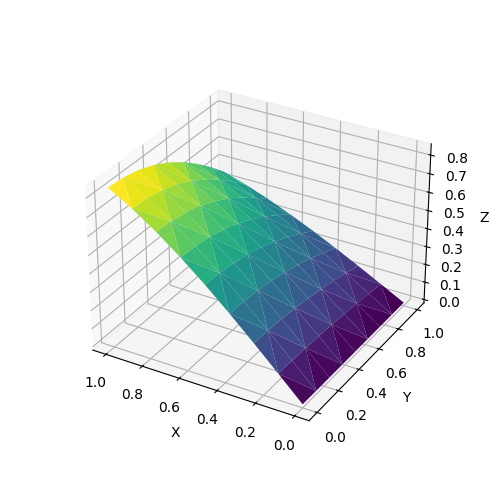
\includegraphics[width=\textwidth]{../../res_bac/res-[data|2-Neumann-regular-a8].png}
      \caption{$n =  8$}
  \end{subfigure}
  \hfill
  \begin{subfigure}[b]{0.18\textwidth}
      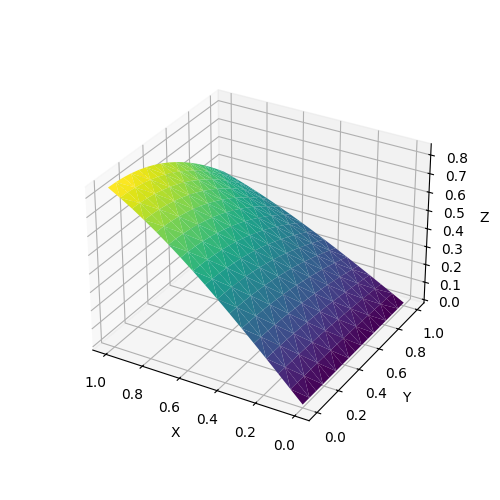
\includegraphics[width=\textwidth]{../../res_bac/res-[data|2-Neumann-regular-b16].png}
      \caption{$n= 16$}
  \end{subfigure}
  \hfill
  \begin{subfigure}[b]{0.18\textwidth}
      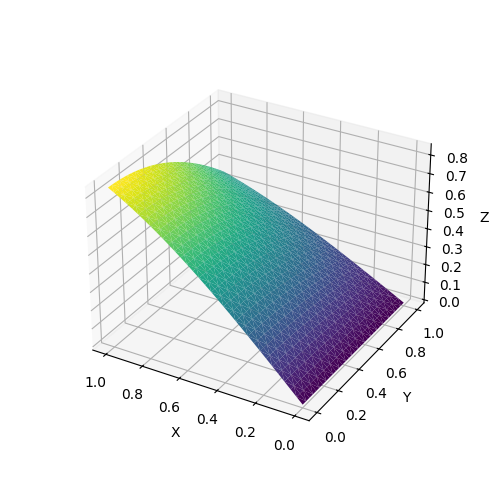
\includegraphics[width=\textwidth]{../../res_bac/res-[data|2-Neumann-regular-c32].png}
      \caption{$n = 32$}
  \end{subfigure}
  \hfill
  \begin{subfigure}[b]{0.18\textwidth}
      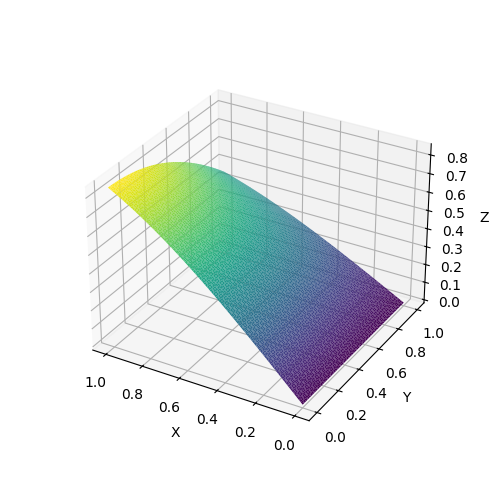
\includegraphics[width=\textwidth]{../../res_bac/res-[data|2-Neumann-regular-d64].png}
      \caption{$n = 64$}
  \end{subfigure}
  \hfill
  \begin{subfigure}[b]{0.18\textwidth}
      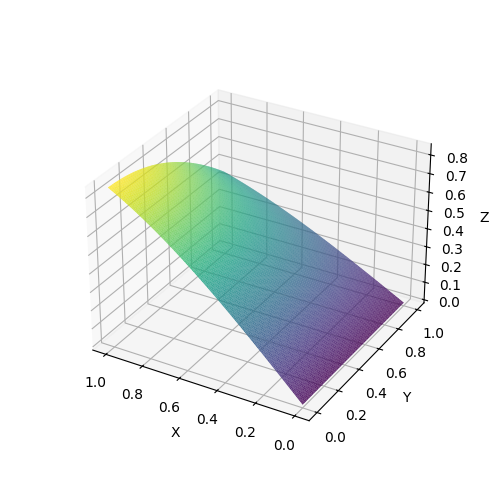
\includegraphics[width=\textwidth]{../../res_bac/res-[data|2-Neumann-regular-e128].png}
      \caption{$n = 128$}
  \end{subfigure}
\end{figure}

误差分析如下表:

\begin{table}[H]
  \centering
  \begin{tabular}{|c|c|c|c|c|c|c|}
  \hline
   & 8 & 16 & 32 & 64 & 128 & convergence rate \\
  \hline
  Norm-1 & 4.1105e-04 & 9.9638e-05 & 2.4385e-05 & 6.0176e-06 & 1.4939e-06 & 2.010 \\
  Norm-2 & 4.9101e-04 & 1.1974e-04 & 2.9409e-05 & 7.2694e-06 & 1.8058e-06 & 2.009 \\
  Norm-$\infty$ & 1.0001e-03 & 2.5429e-04 & 6.3896e-05 & 2.1884e-05 & 7.1384e-06 & 1.616 \\
  \hline
  \end{tabular}
  \end{table}

\subsubsubsection{混合边值条件}

\[
\begin{cases}
  - \Delta u = 2\sin x \cos y, \text{in~~} \Omega \\
  u = \sin x \cos y, x = 0 \\
  \apart{u}{\bm{n}}{} = \cos x \cos y, x = 1 \\  
  u = \sin x \cos y, y = 0 \\
  \apart{u}{\bm{n}}{} = - \sin x \sin y, y = 1 \\  
\end{cases}
\]

求解结果如下图:

\begin{figure}[H]
  \centering
  \begin{subfigure}[b]{0.18\textwidth}
      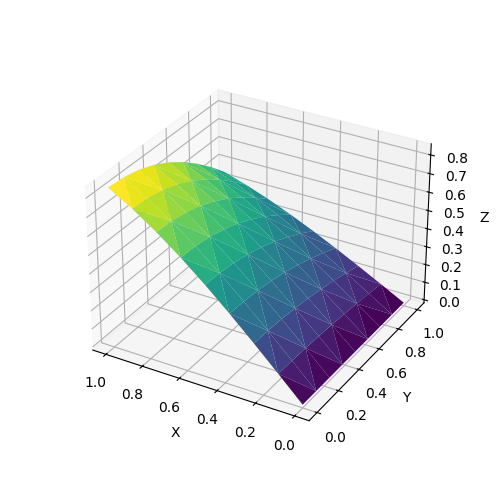
\includegraphics[width=\textwidth]{../../res_bac/res-[data|2-mixed-regular-a8].png}
      \caption{$n =  8$}
  \end{subfigure}
  \hfill
  \begin{subfigure}[b]{0.18\textwidth}
      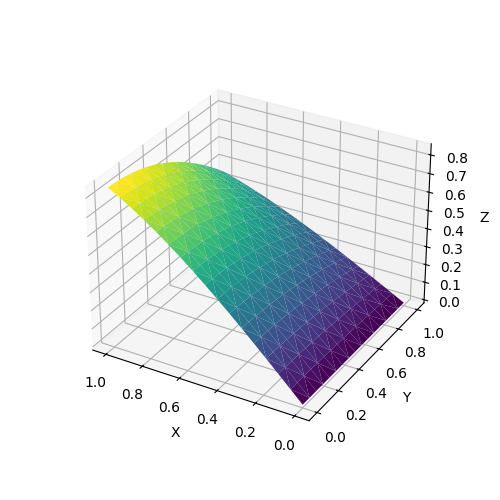
\includegraphics[width=\textwidth]{../../res_bac/res-[data|2-mixed-regular-b16].png}
      \caption{$n= 16$}
  \end{subfigure}
  \hfill
  \begin{subfigure}[b]{0.18\textwidth}
      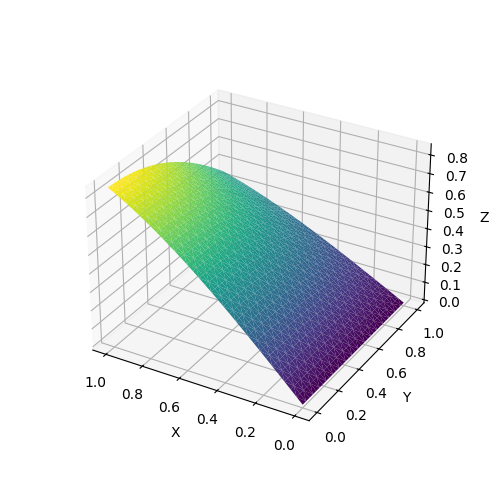
\includegraphics[width=\textwidth]{../../res_bac/res-[data|2-mixed-regular-c32].png}
      \caption{$n = 32$}
  \end{subfigure}
  \hfill
  \begin{subfigure}[b]{0.18\textwidth}
      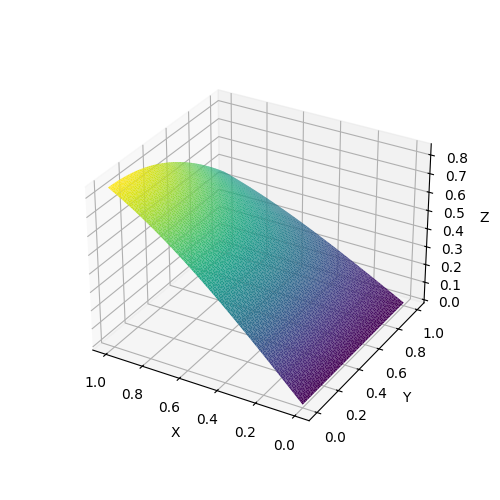
\includegraphics[width=\textwidth]{../../res_bac/res-[data|2-mixed-regular-d64].png}
      \caption{$n = 64$}
  \end{subfigure}
  \hfill
  \begin{subfigure}[b]{0.18\textwidth}
      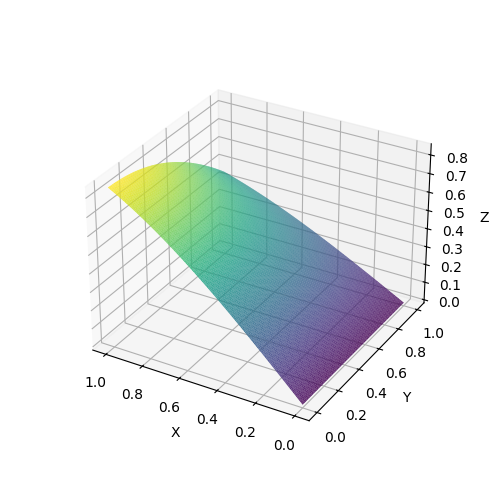
\includegraphics[width=\textwidth]{../../res_bac/res-[data|2-mixed-regular-e128].png}
      \caption{$n = 128$}
  \end{subfigure}
\end{figure}

误差分析如下表:

\begin{table}[H]
  \centering
  \begin{tabular}{|c|c|c|c|c|c|c|}
  \hline
   & 8 & 16 & 32 & 64 & 128 & convergence rate \\
  \hline
  Norm-1 & 1.4342e-04 & 3.5781e-05 & 8.9706e-06 & 2.2493e-06 & 5.6340e-07 & 1.997 \\
  Norm-2 & 2.1146e-04 & 5.1558e-05 & 1.2740e-05 & 3.1678e-06 & 7.8990e-07 & 2.004 \\
  Norm-$\infty$ & 5.8935e-04 & 1.5003e-04 & 3.7585e-05 & 9.4011e-06 & 2.3508e-06 & 1.893 \\
  \hline
  \end{tabular}
  \end{table}

\subsubsection{不规则区域}

取 $D = {(x, y) : (x - 0.41)^2 + (y - 0.55)^2 \le 0.15^2}$

\subsubsubsection{Dirichlet 边值条件}

\[
\begin{cases}
  - \Delta u = 2\sin x \cos y, \text{in~~} \Omega \fxg D \\
  u = \sin x \cos y, \text{on ~~} \partial \Omega \fxg D
\end{cases}
\]

求解结果如下图:

\begin{figure}[H]
  \centering
  \begin{subfigure}[b]{0.18\textwidth}
      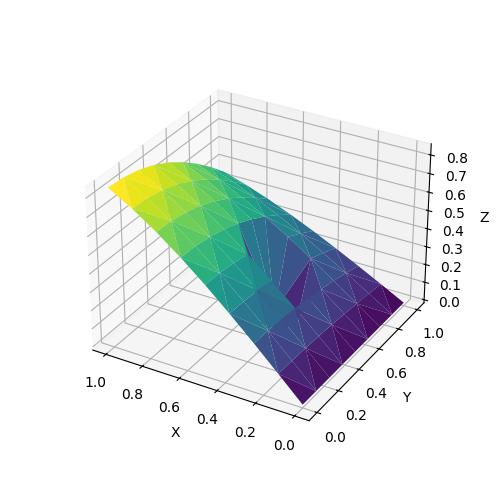
\includegraphics[width=\textwidth]{../../res_bac/res-[data|2-Dirichlet-irregular-a8].png}
      \caption{$n =  8$}
  \end{subfigure}
  \hfill
  \begin{subfigure}[b]{0.18\textwidth}
      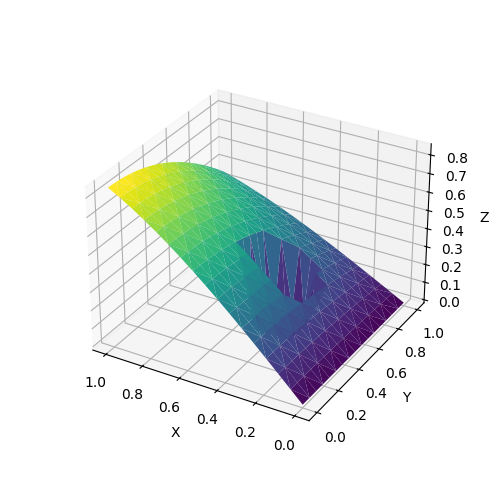
\includegraphics[width=\textwidth]{../../res_bac/res-[data|2-Dirichlet-irregular-b16].png}
      \caption{$n= 16$}
  \end{subfigure}
  \hfill
  \begin{subfigure}[b]{0.18\textwidth}
      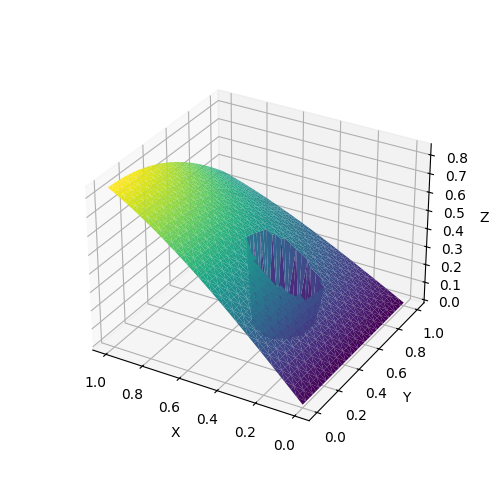
\includegraphics[width=\textwidth]{../../res_bac/res-[data|2-Dirichlet-irregular-c32].png}
      \caption{$n = 32$}
  \end{subfigure}
  \hfill
  \begin{subfigure}[b]{0.18\textwidth}
      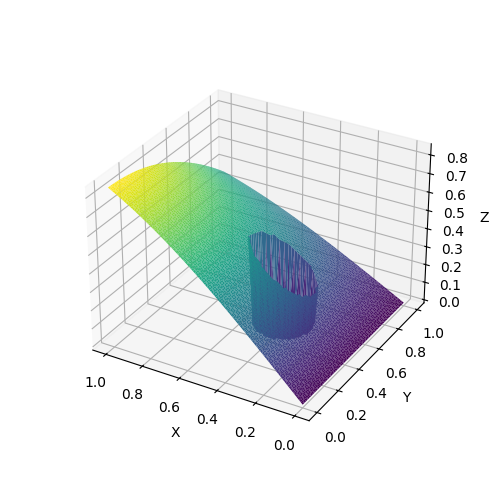
\includegraphics[width=\textwidth]{../../res_bac/res-[data|2-Dirichlet-irregular-d64].png}
      \caption{$n = 64$}
  \end{subfigure}
  \hfill
  \begin{subfigure}[b]{0.18\textwidth}
      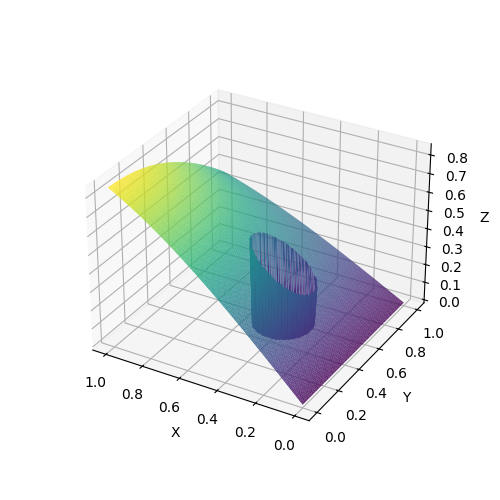
\includegraphics[width=\textwidth]{../../res_bac/res-[data|2-Dirichlet-irregular-e128].png}
      \caption{$n = 128$}
  \end{subfigure}
  \caption{Images of matrices}\label{fig:matrices}
\end{figure}

误差分析如下表:

\begin{table}[H]
  \centering
  \begin{tabular}{|c|c|c|c|c|c|c|}
  \hline
   & 8 & 16 & 32 & 64 & 128 & convergence rate \\
  \hline
  Norm-1 & 1.3171e-04 & 3.2563e-05 & 8.6925e-06 & 2.3375e-06 & 5.7420e-07 & 2.025 \\
  Norm-2 & 1.9844e-04 & 4.5863e-05 & 1.1849e-05 & 3.1519e-06 & 7.6410e-07 & 2.044 \\
  Norm-$\infty$ & 6.0191e-04 & 1.7168e-04 & 4.0499e-05 & 1.2664e-05 & 3.2711e-06 & 1.953 \\
  \hline
  \end{tabular}
  \end{table}

\subsubsubsection{Neumann 边值条件}

\[
\begin{cases}
  - \Delta u = 2\sin x \cos y, \text{in~~} \Omega \fxg D \\
  \apart{u}{\bm{n}}{} = - \cos x \cos y, x = 0 \\
  \apart{u}{\bm{n}}{} = \cos x \cos y, x = 1 \\  
  \apart{u}{\bm{n}}{} = \sin x \sin y, y = 0 \\
  \apart{u}{\bm{n}}{} = - \sin x \sin y, y = 1 \\  
  \apart{u}{\bm{n}}{} = (x - 0.41)/0.15\cdot \cos x \cos y - ( y - 0.55) / 0.15 \sin x \sin y, \text{on~~} \partial D
\end{cases}
\]

求解结果如下图:

\begin{figure}[H]
  \centering
  \begin{subfigure}[b]{0.18\textwidth}
      \includegraphics[width=\textwidth]{../../res_bac/res-[data|2-Neumann-irregular-a8].png}
      \caption{$n =  8$}
  \end{subfigure}
  \hfill
  \begin{subfigure}[b]{0.18\textwidth}
      \includegraphics[width=\textwidth]{../../res_bac/res-[data|2-Neumann-irregular-b16].png}
      \caption{$n= 16$}
  \end{subfigure}
  \hfill
  \begin{subfigure}[b]{0.18\textwidth}
      \includegraphics[width=\textwidth]{../../res_bac/res-[data|2-Neumann-irregular-c32].png}
      \caption{$n = 32$}
  \end{subfigure}
  \hfill
  \begin{subfigure}[b]{0.18\textwidth}
      \includegraphics[width=\textwidth]{../../res_bac/res-[data|2-Neumann-irregular-d64].png}
      \caption{$n = 64$}
  \end{subfigure}
  \hfill
  \begin{subfigure}[b]{0.18\textwidth}
      \includegraphics[width=\textwidth]{../../res_bac/res-[data|2-Neumann-irregular-e128].png}
      \caption{$n = 128$}
  \end{subfigure}
\end{figure}

误差分析如下表:

\begin{table}[H]
  \centering
  \begin{tabular}{|c|c|c|c|c|c|c|}
  \hline
   & 8 & 16 & 32 & 64 & 128 & convergence rate \\
  \hline
  Norm-1 & 4.5160e-04 & 1.3205e-04 & 3.3029e-05 & 7.6640e-06 & 1.9621e-06 & 1.966  \\
  Norm-2 & 5.2538e-04 & 1.5493e-04 & 3.8812e-05 & 9.0439e-06 & 2.3123e-06 & 1.968 \\
  Norm-$\infty$ & 9.9576e-04 & 3.1352e-04 & 9.4772e-05 & 2.9627e-05 & 9.0912e-06 & 1.704 \\
  \hline
  \end{tabular}
  \end{table}

\subsubsubsection{混合边值条件}

\[
\begin{cases}
  - \Delta u = 2\sin x \cos y, \text{in~~} \Omega \fxg D \\
  u = \sin x \cos y, x = 0 \\
  \apart{u}{\bm{n}}{} = \cos x \cos y, x = 1 \\  
  u = \sin x \cos y, y = 0 \\
  \apart{u}{\bm{n}}{} = - \sin x \sin y, y = 1 \\  
  \apart{u}{\bm{n}}{} = (x - 0.41)/0.15\cdot \cos x \cos y - ( y - 0.55) / 0.15 \sin x \sin y, \text{on~~} \partial D
\end{cases}
\]

求解结果如下图:

\begin{figure}[H]
  \centering
  \begin{subfigure}[b]{0.18\textwidth}
      \includegraphics[width=\textwidth]{../../res_bac/res-[data|2-mixed-irregular-a8].png}
      \caption{$n =  8$}
  \end{subfigure}
  \hfill
  \begin{subfigure}[b]{0.18\textwidth}
      \includegraphics[width=\textwidth]{../../res_bac/res-[data|2-mixed-irregular-b16].png}
      \caption{$n= 16$}
  \end{subfigure}
  \hfill
  \begin{subfigure}[b]{0.18\textwidth}
      \includegraphics[width=\textwidth]{../../res_bac/res-[data|2-mixed-irregular-c32].png}
      \caption{$n = 32$}
  \end{subfigure}
  \hfill
  \begin{subfigure}[b]{0.18\textwidth}
      \includegraphics[width=\textwidth]{../../res_bac/res-[data|2-mixed-irregular-d64].png}
      \caption{$n = 64$}
  \end{subfigure}
  \hfill
  \begin{subfigure}[b]{0.18\textwidth}
      \includegraphics[width=\textwidth]{../../res_bac/res-[data|2-mixed-irregular-e128].png}
      \caption{$n = 128$}
  \end{subfigure}
\end{figure}

误差分析如下表:

\begin{table}[H]
  \centering
  \begin{tabular}{|c|c|c|c|c|c|c|}
  \hline
   & 8 & 16 & 32 & 64 & 128 & convergence rate \\
  \hline
  Norm-1 & 3.3837e-04 & 7.6379e-05 & 1.9159e-05 & 4.8952e-06 & 1.2187e-06 & 2.006 \\
  Norm-2 & 4.3877e-04 & 9.4432e-05 & 2.3747e-05 & 6.0061e-06 & 1.4939e-06 & 2.007 \\
  Norm-$\infty$ & 9.2712e-04 & 2.0114e-04 & 5.1790e-05 & 1.3050e-05 & 3.2842e-06 & 1.990 \\
  \hline
  \end{tabular}
  \end{table}

\subsection{测试样例3}

\[
  u(x, y) = \ln (1 + x^2 + y^2), \Omega = [0, 1]^2
\]


\subsubsection{规则区域}

\subsubsubsection{Dirichlet 边值条件}

\[
\begin{cases}
  - \Delta u = \frac{4x^2 + 4y^2 - 4(1 + x^2 + y^2)}{(1 + x^2 + y^2)^2}, \text{in~~} \Omega\\
  u = \ln (1 + x^2 + y^2), \text{on ~~} \partial \Omega
\end{cases}
\]

求解结果如下图:

\begin{figure}[H]
  \centering
  \begin{subfigure}[b]{0.18\textwidth}
      \includegraphics[width=\textwidth]{../../res_bac/res-[data|3-Dirichlet-regular-a8].png}
      \caption{$n =  8$}
  \end{subfigure}
  \hfill
  \begin{subfigure}[b]{0.18\textwidth}
      \includegraphics[width=\textwidth]{../../res_bac/res-[data|3-Dirichlet-regular-b16].png}
      \caption{$n= 16$}
  \end{subfigure}
  \hfill
  \begin{subfigure}[b]{0.18\textwidth}
      \includegraphics[width=\textwidth]{../../res_bac/res-[data|3-Dirichlet-regular-c32].png}
      \caption{$n = 32$}
  \end{subfigure}
  \hfill
  \begin{subfigure}[b]{0.18\textwidth}
      \includegraphics[width=\textwidth]{../../res_bac/res-[data|3-Dirichlet-regular-d64].png}
      \caption{$n = 64$}
  \end{subfigure}
  \hfill
  \begin{subfigure}[b]{0.18\textwidth}
      \includegraphics[width=\textwidth]{../../res_bac/res-[data|3-Dirichlet-regular-e128].png}
      \caption{$n = 128$}
  \end{subfigure}
\end{figure}

误差分析如下表:

\begin{table}[H]
  \centering
  \begin{tabular}{|c|c|c|c|c|c|c|}
  \hline
   & 8 & 16 & 32 & 64 & 128 & convergence rate \\
  \hline
  Norm-1 & 5.6732e-05 & 1.6262e-05 & 4.3446e-06 & 1.1212e-06 & 2.8480e-07 & 1.978 \\
  Norm-2 & 9.7012e-05 & 2.5774e-05 & 6.6373e-06 & 1.6845e-06 & 4.2440e-07 & 1.996 \\
  Norm-$\infty$ & 3.1321e-04 & 7.9810e-05 & 2.0340e-05 & 5.0917e-06 & 1.2741e-06 & 1.999 \\
  \hline
  \end{tabular}
  \end{table}

\subsubsubsection{Neumann 边值条件}

\[
\begin{cases}
  - \Delta u = \frac{4x^2 + 4y^2 - 4(1 + x^2 + y^2)}{(1 + x^2 + y^2)^2}, \text{in~~} \Omega\\
  \apart{u}{\bm{n}}{} = -\frac{2x}{1+x^2+y^2}, x = 0 \\
  \apart{u}{\bm{n}}{} = \frac{2x}{1+x^2+y^2}, x = 1 \\  
  \apart{u}{\bm{n}}{} = -\frac{2y}{1+x^2+y^2}, y = 0 \\
  \apart{u}{\bm{n}}{} = \frac{2y}{1+x^2+y^2}, y = 1 \\ 
\end{cases}
\]

求解结果如下图:

\begin{figure}[H]
  \centering
  \begin{subfigure}[b]{0.18\textwidth}
      \includegraphics[width=\textwidth]{../../res_bac/res-[data|3-Neumann-regular-a8].png}
      \caption{$n =  8$}
  \end{subfigure}
  \hfill
  \begin{subfigure}[b]{0.18\textwidth}
      \includegraphics[width=\textwidth]{../../res_bac/res-[data|3-Neumann-regular-b16].png}
      \caption{$n= 16$}
  \end{subfigure}
  \hfill
  \begin{subfigure}[b]{0.18\textwidth}
      \includegraphics[width=\textwidth]{../../res_bac/res-[data|3-Neumann-regular-c32].png}
      \caption{$n = 32$}
  \end{subfigure}
  \hfill
  \begin{subfigure}[b]{0.18\textwidth}
      \includegraphics[width=\textwidth]{../../res_bac/res-[data|3-Neumann-regular-d64].png}
      \caption{$n = 64$}
  \end{subfigure}
  \hfill
  \begin{subfigure}[b]{0.18\textwidth}
      \includegraphics[width=\textwidth]{../../res_bac/res-[data|3-Neumann-regular-e128].png}
      \caption{$n = 128$}
  \end{subfigure}
\end{figure}

误差分析如下表:

\begin{table}[H]
  \centering
  \begin{tabular}{|c|c|c|c|c|c|c|}
  \hline
   & 8 & 16 & 32 & 64 & 128 & convergence rate \\
  \hline
  Norm-1 & 1.4097e-03 & 3.4745e-04 & 8.5509e-05 & 2.1146e-05 & 5.2523e-06 & 2.009 \\
  Norm-2 & 1.7683e-03 & 4.4031e-04 & 1.0881e-04 & 2.6930e-05 & 6.6869e-06 & 2.010 \\
  Norm-$\infty$ & 4.8837e-03 & 1.5048e-03 & 4.4405e-04 & 1.2779e-04 & 3.6117e-05 & 1.823 \\
  \hline
  \end{tabular}
  \end{table}

\subsubsubsection{混合边值条件}

\[
\begin{cases}
  - \Delta u = \frac{4x^2 + 4y^2 - 4(1 + x^2 + y^2)}{(1 + x^2 + y^2)^2}, \text{in~~} \Omega\\
  \apart{u}{\bm{n}}{} = -\frac{2x}{1+x^2+y^2}, x = 0 \\
  \apart{u}{\bm{n}}{} = \frac{2x}{1+x^2+y^2}, x = 1 \\  
  u = \ln (1 + x^2 + y^2), y = 0 \\
  u = \ln (1 + x^2 + y^2), y = 1 \\  
\end{cases}
\]

求解结果如下图:

\begin{figure}[H]
  \centering
  \begin{subfigure}[b]{0.18\textwidth}
      \includegraphics[width=\textwidth]{../../res_bac/res-[data|3-mixed-regular-a8].png}
      \caption{$n =  8$}
  \end{subfigure}
  \hfill
  \begin{subfigure}[b]{0.18\textwidth}
      \includegraphics[width=\textwidth]{../../res_bac/res-[data|3-mixed-regular-b16].png}
      \caption{$n= 16$}
  \end{subfigure}
  \hfill
  \begin{subfigure}[b]{0.18\textwidth}
      \includegraphics[width=\textwidth]{../../res_bac/res-[data|3-mixed-regular-c32].png}
      \caption{$n = 32$}
  \end{subfigure}
  \hfill
  \begin{subfigure}[b]{0.18\textwidth}
      \includegraphics[width=\textwidth]{../../res_bac/res-[data|3-mixed-regular-d64].png}
      \caption{$n = 64$}
  \end{subfigure}
  \hfill
  \begin{subfigure}[b]{0.18\textwidth}
      \includegraphics[width=\textwidth]{../../res_bac/res-[data|3-mixed-regular-e128].png}
      \caption{$n = 128$}
  \end{subfigure}
\end{figure}

误差分析如下表:

\begin{table}[H]
  \centering
  \begin{tabular}{|c|c|c|c|c|c|c|}
  \hline
   & 8 & 16 & 32 & 64 & 128 & convergence rate \\
  \hline
  Norm-1 & 2.9619e-04 & 7.3878e-05 & 1.8468e-05 & 4.6196e-06 & 1.1555e-06 &  1.999 \\
  Norm-2 & 4.0336e-04 & 9.8126e-05 & 2.4186e-05 & 6.0043e-06 & 1.4960e-06 &  2.005 \\
  Norm-$\infty$ & 1.0211e-03 & 2.5788e-04 & 6.4686e-05 & 1.6187e-05 & 4.0473e-06 & 2.000 \\
  \hline
  \end{tabular}
  \end{table}

\subsubsection{不规则区域}

取 $D = {(x, y) : (x - 0.41)^2 + (y - 0.55)^2 \le 0.15^2}$

\subsubsubsection{Dirichlet 边值条件}

\[
\begin{cases}
  - \Delta u = \frac{4x^2 + 4y^2 - 4(1 + x^2 + y^2)}{(1 + x^2 + y^2)^2}, \text{in~~} \Omega \fxg D \\
  u = \ln (1 + x^2 + y^2), \text{on ~~} \partial \Omega \fxg D
\end{cases}
\]

求解结果如下图:

\begin{figure}[H]
  \centering
  \begin{subfigure}[b]{0.18\textwidth}
      \includegraphics[width=\textwidth]{../../res_bac/res-[data|3-Dirichlet-irregular-a8].png}
      \caption{$n =  8$}
  \end{subfigure}
  \hfill
  \begin{subfigure}[b]{0.18\textwidth}
      \includegraphics[width=\textwidth]{../../res_bac/res-[data|3-Dirichlet-irregular-b16].png}
      \caption{$n= 16$}
  \end{subfigure}
  \hfill
  \begin{subfigure}[b]{0.18\textwidth}
      \includegraphics[width=\textwidth]{../../res_bac/res-[data|3-Dirichlet-irregular-c32].png}
      \caption{$n = 32$}
  \end{subfigure}
  \hfill
  \begin{subfigure}[b]{0.18\textwidth}
      \includegraphics[width=\textwidth]{../../res_bac/res-[data|3-Dirichlet-irregular-d64].png}
      \caption{$n = 64$}
  \end{subfigure}
  \hfill
  \begin{subfigure}[b]{0.18\textwidth}
      \includegraphics[width=\textwidth]{../../res_bac/res-[data|3-Dirichlet-irregular-e128].png}
      \caption{$n = 128$}
  \end{subfigure}
  \caption{Images of matrices}\label{fig:matrices}
\end{figure}

误差分析如下表:

\begin{table}[H]
  \centering
  \begin{tabular}{|c|c|c|c|c|c|c|}
  \hline
   & 8 & 16 & 32 & 64 & 128 & convergence rate \\
  \hline
  Norm-1 & 3.3287e-04 & 9.1638e-05 & 2.2958e-05 & 6.1440e-06 & 1.4888e-06 & 2.045 \\
  Norm-2 & 5.0075e-04 & 1.3545e-04 & 3.2453e-05 & 8.6333e-06 & 2.0749e-06 & 2.057 \\
  Norm-$\infty$ & 1.3518e-03 & 4.8945e-04 & 1.3315e-04 & 3.4820e-05 & 9.1099e-06 & 1.934 \\
  \hline
  \end{tabular}
  \end{table}

\subsubsubsection{Neumann 边值条件}

\[
\begin{cases}
  - \Delta u = \frac{4x^2 + 4y^2 - 4(1 + x^2 + y^2)}{(1 + x^2 + y^2)^2}, \text{in~~} \Omega \fxg D \\
  \apart{u}{\bm{n}}{} = -\frac{2x}{1+x^2+y^2}, x = 0 \\
  \apart{u}{\bm{n}}{} = \frac{2x}{1+x^2+y^2}, x = 1 \\  
  \apart{u}{\bm{n}}{} = -\frac{2y}{1+x^2+y^2}, y = 0 \\
  \apart{u}{\bm{n}}{} = \frac{2y}{1+x^2+y^2}, y = 1 \\ 
  \apart{u}{\bm{n}}{} = (x - 0.41)/0.15\cdot\frac{2x}{1+x^2+y^2} + ( y - 0.55) / 0.15 \frac{2y}{1+x^2+y^2}, \text{on~~} \partial D
\end{cases}
\]

求解结果如下图:

\begin{figure}[H]
  \centering
  \begin{subfigure}[b]{0.18\textwidth}
      \includegraphics[width=\textwidth]{../../res_bac/res-[data|3-Neumann-irregular-a8].png}
      \caption{$n =  8$}
  \end{subfigure}
  \hfill
  \begin{subfigure}[b]{0.18\textwidth}
      \includegraphics[width=\textwidth]{../../res_bac/res-[data|3-Neumann-irregular-b16].png}
      \caption{$n= 16$}
  \end{subfigure}
  \hfill
  \begin{subfigure}[b]{0.18\textwidth}
      \includegraphics[width=\textwidth]{../../res_bac/res-[data|3-Neumann-irregular-c32].png}
      \caption{$n = 32$}
  \end{subfigure}
  \hfill
  \begin{subfigure}[b]{0.18\textwidth}
      \includegraphics[width=\textwidth]{../../res_bac/res-[data|3-Neumann-irregular-d64].png}
      \caption{$n = 64$}
  \end{subfigure}
  \hfill
  \begin{subfigure}[b]{0.18\textwidth}
      \includegraphics[width=\textwidth]{../../res_bac/res-[data|3-Neumann-irregular-e128].png}
      \caption{$n = 128$}
  \end{subfigure}
\end{figure}

误差分析如下表:

\begin{table}[H]
  \centering
  \begin{tabular}{|c|c|c|c|c|c|c|}
  \hline
   & 8 & 16 & 32 & 64 & 128 & convergence rate \\
  \hline
  Norm-1 & 1.5712e-03 & 3.6338e-04 & 9.8442e-05 & 2.3558e-05 & 6.3243e-06 & 1.897 \\
  Norm-2 & 1.9066e-03 & 4.4298e-04 & 1.2130e-04 & 2.8952e-05 & 7.8485e-06 & 1.883 \\
  Norm-$\infty$ & 4.9056e-03 & 1.3201e-03 & 4.6083e-04 & 1.2257e-04 & 4.1674e-05 & 1.556 \\
  \hline
  \end{tabular}
  \end{table}

\subsubsubsection{混合边值条件}

\[
\begin{cases}
  - \Delta u = \frac{4x^2 + 4y^2 - 4(1 + x^2 + y^2)}{(1 + x^2 + y^2)^2}, \text{in~~} \Omega \fxg D \\
  \apart{u}{\bm{n}}{} = -\frac{2x}{1+x^2+y^2}, x = 0 \\
  \apart{u}{\bm{n}}{} = \frac{2x}{1+x^2+y^2}, x = 1 \\  
  u = \ln (1 + x^2 + y^2), y = 0 \\
  u = \ln (1 + x^2 + y^2), y = 1 \\  
  u = \ln (1 + x^2 + y^2), \text{on~~} \partial D
\end{cases}
\]


求解结果如下图:

\begin{figure}[H]
  \centering
  \begin{subfigure}[b]{0.18\textwidth}
      \includegraphics[width=\textwidth]{../../res_bac/res-[data|3-mixed-irregular-a8].png}
      \caption{$n =  8$}
  \end{subfigure}
  \hfill
  \begin{subfigure}[b]{0.18\textwidth}
      \includegraphics[width=\textwidth]{../../res_bac/res-[data|3-mixed-irregular-b16].png}
      \caption{$n= 16$}
  \end{subfigure}
  \hfill
  \begin{subfigure}[b]{0.18\textwidth}
      \includegraphics[width=\textwidth]{../../res_bac/res-[data|3-mixed-irregular-c32].png}
      \caption{$n = 32$}
  \end{subfigure}
  \hfill
  \begin{subfigure}[b]{0.18\textwidth}
      \includegraphics[width=\textwidth]{../../res_bac/res-[data|3-mixed-irregular-d64].png}
      \caption{$n = 64$}
  \end{subfigure}
  \hfill
  \begin{subfigure}[b]{0.18\textwidth}
      \includegraphics[width=\textwidth]{../../res_bac/res-[data|3-mixed-irregular-e128].png}
      \caption{$n = 128$}
  \end{subfigure}
\end{figure}

误差分析如下表:

\begin{table}[H]
  \centering
  \begin{tabular}{|c|c|c|c|c|c|c|}
  \hline
   & 8 & 16 & 32 & 64 & 128 & convergence rate \\
  \hline
  Norm-1 & 5.0856e-04 & 1.4095e-04 & 3.4098e-05 & 8.8528e-06 & 2.1579e-06 & 2.037 \\
  Norm-2 & 6.7817e-04 & 1.8896e-04 & 4.5625e-05 & 1.1839e-05 & 2.8953e-06 & 2.032 \\
  Norm-$\infty$ & 1.4730e-03 & 4.9732e-04 & 1.3796e-04 & 3.5208e-05 & 9.2004e-06 & 1.936 \\
  \hline
  \end{tabular}
  \end{table}


\subsection{总结}

根据测试样例的结果,可以看出,收敛率基本都在2附近,与理论收敛率相符。

\nocite{*}
\printbibliography[heading=bibintoc, title=\ebibname]

\end{document}